\documentclass[titlepage,12pt,twoside,a4paper]{report}

\usepackage[utf8]{inputenc}
\usepackage[english]{babel}
\usepackage{pdfcolmk}
\usepackage{graphicx}
\usepackage{epstopdf}
\usepackage{adjustbox}
\usepackage{amsmath,amssymb}
\usepackage{bm}
\usepackage{amstext}
\usepackage{amsthm}
\usepackage{rotating}
\usepackage{enumerate}
\usepackage{epigraph}
\usepackage[backend=bibtex,style=chem-acs,natbib=true,doi=true,isbn=false,url=true,arxiv=false]{biblatex}
\addbibresource{./library}
\usepackage[breaklinks]{hyperref}
\hypersetup{
    colorlinks=true,
    citecolor=red,
    filecolor=black,
    linkcolor=cyan,
    urlcolor=blue
}
\usepackage{multirow}
\usepackage[usenames,dvipsnames]{color}
\usepackage{verbatim}
\usepackage{float}
\usepackage{url}
\usepackage{lscape}
\usepackage{afterpage}
\usepackage{longtable}
\usepackage[font=small,labelfont=bf]{caption}
\usepackage{pdfpages}
\usepackage[utf8]{inputenc}
\usepackage[english]{babel}
\usepackage{parskip,array,booktabs}
\raggedbottom
\DeclareUnicodeCharacter{2212}{-}
\DeclareUnicodeCharacter{0301}{\'{e}}
\usepackage{listings}
\usepackage{color}
\usepackage{appendix}
\usepackage{blindtext}
\usepackage{tikz}

%%%%%%%%%%%%%%%%%%%%%%%
%% PAGE SETUP        %%
%%%%%%%%%%%%%%%%%%%%%%%
\usepackage{geometry}
\geometry{paper=a4paper,            % scientific thesis standard
            left=3cm,
            right=2.5cm,
            top=3cm,
            bottom=3cm,
 }
\setlength{\headheight}{27.2pt}
\bibliography{library}

\usepackage{fancyhdr}
\fancyhead{}
\fancyhead[LO]{\slshape \rightmark}
\fancyhead[RO,LE]{\textbf{\thepage}}
\fancyhead[RE]{\slshape \leftmark}
\fancyfoot{}
\pagestyle{fancy}

\makeatletter
\makeatother

\def\blankpage{%
      \clearpage%
      \thispagestyle{empty}%
      \addtocounter{page}{-1}%
      \null%
      \clearpage}

%%%%%%%%%%%%%%%%%%%%%%%
%% NEW COMMANDS      %%
%%%%%%%%%%%%%%%%%%%%%%%
\renewcommand{\chaptermark}[1]{\markboth{\chaptername \ \thechapter \ \ #1}{}}
\renewcommand{\sectionmark}[1]{\markright{\thesection \ \ #1}}
\renewcommand{\eqref}[1]{\textup{\color{cyan} {\normalfont(\ref{#1}}\normalfont)}}
\newcommand{\figref}[1]{\hyperref[#1]{Fig.~\ref*{#1}}}
\newcommand{\figrefi}[2]{\hyperref[#1]{Fig.~\ref*{#1}~#2}}
\newcommand{\figrefs}[1]{\hyperref[#1]{Figs.~\ref*{#1}}}
\newcommand{\figrefn}[2]{\hyperref[#1]{Figs.~\ref*{#1}~#2}}
\newcommand{\figrefni}[2]{\hyperref[#1]{Figs.~\ref*{#1}--#2}}
\newcommand{\tabref}[1]{\hyperref[#1]{Table~\ref*{#1}}}
\newcommand{\tabrefn}[1]{\hyperref[#1]{Tables~\ref*{#1}}}
\newcommand{\secref}[1]{\hyperref[#1]{Section~\ref*{#1}}}
\newcommand{\appref}[1]{\hyperref[#1]{Appendix~\ref*{#1}}}
\newcommand{\chapref}[1]{\hyperref[#1]{Chapter~\ref*{#1}}}

\newcommand{\chapquote}[3]{\begin{quotation}\textit{#1}\end{quotation} \begin{flushright}#2\end{flushright}}

\newcommand{\angs}{\textup{\AA}}
\newcommand{\Rmin}{$R_{\text{min}}$}
\newcommand{\spring}{kcal/mol/\AA{}\textsuperscript{2}}
\newcommand{\prim}{\textsuperscript{$\prime$}}
\newcommand{\dprim}{\textsuperscript{$\prime\prime$}}
\newcommand{\Na}{Na$^+$}
\newcommand{\K}{K$^+$}
\newcommand{\Hi}{H$^+$}
\newcommand{\Cl}{Cl$^-$}
\newcommand{\Ca}{Ca$^{2+}$}
\newcommand{\Tl}{Tl$^+$}
\newcommand{\GltPh}{Glt$_\text{Ph}$}
\newcommand{\GltTk}{Glt$_\text{Tk}$}
\newcommand{\pka}{p\textit{K}\textsubscript{a}}
\newcommand{\kT}{k_{\text{B}}T}

\begin{document}
%%%%%%%%%%%%%%%%%%%%%%%
%% PREAMBLE TEXT     %%
%%%%%%%%%%%%%%%%%%%%%%%
\pagenumbering{roman}

\begin{titlepage}

\begin{center}

\vspace*{0.1in}

\begin{LARGE}
Computer Modelling the Root Cause of  \\ 
\end{LARGE}
\vspace*{0.1in}
\begin{LARGE}
Cystic Fibrosis
\end{LARGE}
\begin{large} \\
\vspace{0.1in}
by Miro Alexander Astore

%\vspace{0.1in}
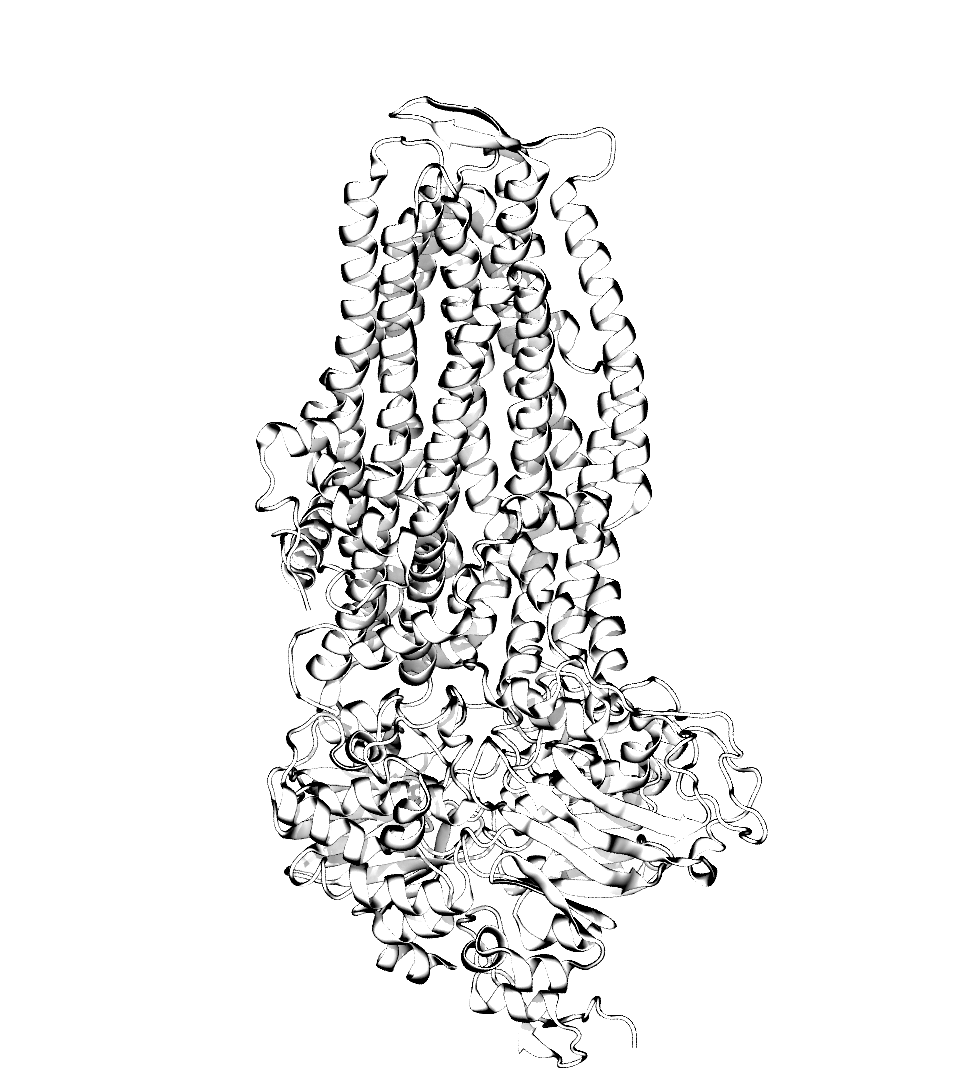
\includegraphics[width=0.8\textwidth]{figures/skeleton_bw.png}
%\vspace{0.1in}
%TO\\
%\vspace{0.1in}
%THE
%{\Large F}ACULTY OF {\Large S}CIENCE\\
\vspace{-0.05in}

\textit{A thesis submitted in fulfilment of the}\\
\textit{requirements for the degree of}

%IN PARTIAL FULFILMENT OF THE REQUIREMENTS\\
%FOR THE DEGREE OF \\
%{\Large D}OCTOR OF {\Large P}HILOSOPHY\\
%IN THE SUBJECT OF \\
%{\Large B}IOPHYSICS\\
\vspace{0.1in}

%\begin{large}
Doctor of Philosophy
%\end{large}

\vspace{0.1in}

%\begin{large}
The School of Physics\\
Faculty of Science\\
The University of Sydney\\
2022
%\vspace{0.05in}
%\end{large}

%\vspace{0.05in}
\end{large}

\end{center}
\end{titlepage}

%=======================================================================================%
\newpage
\begin{center}
Declaration of Original contribution

\vspace{0.5in}

of the dissertation submitted by

\vspace{0.25in}

Miro Alexander Astore

\end{center}

\vspace{0.5in}

\noindent This is to certify that to the best of my knowledge, the content of this 
thesis is my own work. This thesis has not been submitted for any degree or other 
purposes.

\noindent I certify that the intellectual content of this thesis is the product of 
my own work and that all the assistance received in preparing this thesis and sources 
have been acknowledged.

\vspace{1in}

% \begin{tikzpicture}[remember picture,overlay]
%     \node[xshift=4cm,yshift=-14.0cm,anchor=north west] at (current page.north west){%
%     \includegraphics[width=35mm]{Figures/signature-JS.jpg}};
% \end{tikzpicture}

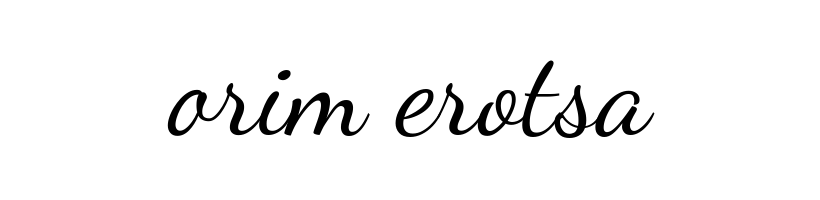
\includegraphics[width=6cm]{figures/signatures/orim_sig_fake.png} \hspace{3.0cm} 09/09/2022\\
% \hspace{12cm} {\large 15/03/2019} \\
\noindent \line(1,0){225} \hspace{1.0cm} \line(1,0){140} \\
 {\em Miro Alexander Astore}, Author \hspace{3.65cm} Date
%=======================================================================================%

%=======================================================================================%
\begin{abstract}
\setcounter{page}{3}
\thispagestyle{plain}

Cystic Fibrosis is the most common fatal genetic condition in Caucasian populations. It is a debilitating disease, significantly shortening the life span of patients and degrading their quality of life. It is caused by deleterious mutations to a protein known as the Cystic Fibrosis Transmembrane conductance Regulator (CFTR). This protein acts as an anion channel.

Over the last decade there have been an increasing number of clinically approved small molecule drugs which act directly on CFTR in order to restore its function. These drugs are called CFTR modulators. Unfortunately, since CF is a rare disease and there are more than 400 mutations which cause it, it is currently unclear which mutations will respond to modulator therapy. This leaves many patients with under studied mutations unable to access modulator therapy.

In this work we performed extensive molecular dynamics (MD) and free energy calculations in order to characterise the many different ways that the CFTR can misfunction. This was done in close collaboration with \textit{in vitro} and clinical experiments in order to understand what types of molecular defects may be treated by existing medications. This work will help more patients access modulator therapy.

We found that rare CFTR mutations exhibit a wide range of molecular defects and that these defects appear to respond to these modulator drugs. The combination of MD, a basic biophysical technique with wet lab studies signals the increasing capability of quantitative physical techniques in biological research.
\end{abstract}

%=======================================================================================%
\newpage


\thispagestyle{empty}


\begin{center}
	\vspace*{\fill}
\textit {In loving memory of Madeline Jennifer Dell} \\
	\vspace*{\fill}
\end{center}
\chapquote{``Fear cuts deeper than swords."}{Arya Stark}

\clearpage

\begin{center}
\begin{Large}
\begin{bfseries}
Acknowledgments
\end{bfseries}
\end{Large}
\end{center}
 Daniel Golestan, a wise man, once told me that to be given the opportunity to create this thesis was a gift. It was. It was a gift given to me by every friend, colleague, teacher, mentor and family member I've spent any time with. The list that follows of those to thank is not complete. If it was you'd be reading about a conversation I had with a middle aged public servant in a hostel north of San Francisco, but that has little to do with Cystic Fibrosis. 

To my parents raised me with not only academic rigor in mind but also a respect for aesthetics which has served me strangely well. I've never had a talent for the creative side of things compared to quantitative disciplines. But were it not for their demand for respect for the arts I'd have remained illiterate. 

To Jeffry for his tutelage and patience, even from across the pacific ocean. 

To Poker. I am a better human being in every conceivable way for having known you. Your wisdom, intelligence and kindness are boundless. You have taught me an inordinate number of things. And yes, I do mean inordinate. 

Nono and Nona I don't think you'll ever read this. I'm sad that you won't understand what I've done but I think you'd be proud if you did. Living in Condell park did more for me than you could know. Far from war torn Beirut or dirt poor Orria I'm sitting in a well lit office writing this with a full stomach and few worries. Sometimes this luck makes my head spin. 

To the whole Waters lab and Shafagh Waters in particular. For your vision, your drive and all your advice. You brought me a truly fascinating PhD project and I benefited greatly from your mentorship. Bridging the gap between cell biology and molecular physics is something that will happen more in the future and I'm lucky to have met such a driven lab to teach me to do so. 

To Serdar, a brilliant mind and a patient boss. Thank you for giving me the best possible experience at grad school I could have asked for. Your willingness to let me pursue self directed projects with a guided hand is a privilege during a PhD and I'm all the better for having gotten it from one of the best. I'm excited to carry some of your physical insight into biological systems to future research projects. 

Maddy, I miss you every day. You couldn't have imagined what it was like to do this after losing you. I carry much of you with me and I wish I had more. I miss your intelligence, your warmth and your love.

You're all in my Loop and I hope I'm in yours.

%=======================================================================================%

%=======================================================================================%
\newpage

\vspace{3in}

\begin{center}
\begin{Large}
\begin{bfseries}
Permission for the Inclusion of Published Work
\end{bfseries}
\end{Large}
\end{center}

\vspace{0.3in}
%The contents of the following chapters are published. \\
%\hspace{\parindent}MA - Miro Alexander Astore \\
%\hspace{\parindent} SK - Serdar Kuyucak \\


\begin{center}
	
\includegraphics [width=\textwidth]{figures/shafa_letter_inclusion_of_published_work.pdf}
\end{center}

\newpage
\begin{center}
\begin{Large}
\begin{bfseries}
Publication Authorship Attribution
\end{bfseries}
\end{Large}
\end{center}

\vspace{0.3in}
\noindent In addition to the statements above, in cases where I am not the 
corresponding author of a published item, permission to include the published 
material has been granted by the corresponding author.

\vspace{1.in}

% \begin{tikzpicture}[remember picture,overlay]
%     \node[xshift=4cm,yshift=-9.0cm,anchor=north west] at (current page.north west){%
%     \includegraphics[width=35mm]{Figures/signature-JS.jpg}};
% \end{tikzpicture}

% \hspace{12cm} {\large 15/03/2019} \\

\includegraphics[width=6cm]{figures/miro_signature.png} \hspace{3.0cm} 09/09/2022\\
\noindent \line(1,0){225} \hspace{1.0cm} \line(1,0){140} \\
 {\em Miro Alexander Astore}, Student \hspace{3.65cm} Date
 
 \vspace{1in}

\noindent As the supervisor for the candidature upon which this thesis is based, 
I can confirm that the authorship attribution statements above are correct.

\vspace{1in}

% \begin{tikzpicture}[remember picture,overlay]
%     \node[xshift=3.5cm,yshift=-19cm,anchor=north west] at (current page.north west){%
%     \includegraphics[width=60mm]{Figures/signature-SK.jpg}};
% \end{tikzpicture}

% \hspace{12cm} {\large 15/03/2019} \\

\includegraphics[width=6cm]{figures/serdar_signature.png} \hspace{3.0cm} 09/09/2022\\
\noindent \line(1,0){225} \hspace{1.0cm} \line(1,0){140} \\
{\em Serdar Kuyucak}, Supervisor \hspace{5.7cm} Date
%=======================================================================================%


%%%%%%%%%%%%%%%%%%%%%%%
%% TABLE OF CONTENTS %%
%%%%%%%%%%%%%%%%%%%%%%%
{
\hypersetup{linkcolor=black}
\tableofcontents
}

\addcontentsline{toc}{chapter}{\hyperref[chap:abbrev]{List of Abbreviations}}
%=======================================================================================%
\chapter*{List of Abbreviations}
\label{chap:abbrev}

\begin{center}
\begin{bfseries}
\newcommand\nomenclature[2]{#1 & #2 \\}
\begin{longtable}{@{}p{3cm}@{}p{\dimexpr\textwidth-1cm\relax}@{}}
\nomenclature{${\small AMBER}$}    {Assisted Model Building with Energy Refinement}
\nomenclature{${\small ABC transporter}$}  {ATP-Binding Cassette transporter}
\nomenclature{${\small ATP}$}      {Adenosine Tri-Phosphate}
\nomenclature{${\small BAR}$}      {Bennett-Acceptance-Ratio}
\nomenclature{${\small CF}$}        {Cystic Fibrosis}
\nomenclature{${\small CFTR}$}      {Cystic Fibrosis Transmembrane Conductance Regulator, also abbreviated ABCC7}
\nomenclature{${\small CHARMM}$}   {Chemistry at Harvard Macromolecular Mechanics}
\nomenclature{${\small CMAP}$}     {energy grid correction map}
\nomenclature{${\small COM}$}      {Centre of Mass}
\nomenclature{${\small Cryo-EM}$}  {Cryogenic Electron Microscopy}
\nomenclature{${\small CV}$}       {Collective Variable}
\nomenclature{${\small DMSO}$}     {Dimethyl Sulfoxide}
\nomenclature{${\small DNA}$}     {Deoxyribose Nucleic Acid}
\nomenclature{${\small FEP}$}      {Free-Energy Perturbation}
\nomenclature{${\small FEV1\%}$}   {Forced Expiratory Volume in 1 second}
\nomenclature{${\small FES\%}$}    {Free Energy Surface}
\nomenclature{${\small FIS}$}      {Forskolin-Induced Swelling}
\nomenclature{${\small gA}$}       {Gramicidin A Ion Channel}
\nomenclature{${\small GROMACS}$}  {GROningen MAchine for Chemical Simulations - MD program}
\nomenclature{${\small GROMOS}$}   {GROningen MOlecular Simulation - MD program}
\nomenclature{${\small iPCR}$}     {inverse Polymerase Chain Reaction}
\nomenclature{${\small iPSCs}$}    {induced Pluripotent Stem Cells}
\nomenclature{${\small LJ}$}       {Lenard-Jones}
\nomenclature{${\small MBAR}$}     {Multistate Bennett-Acceptance-Ratio}
\nomenclature{${\small MD}$}       {Molecular Dynamics}
\nomenclature{${\small MM}$}       {Molecular Mechanics}
\nomenclature{${\small MetaD}$}    {Metadynamics}
\nomenclature{${\small WT-MetaD}$} {Well-Tempered Metadynamics}
\nomenclature{${\small NAMD}$}     {Nanoscale Molecular Dynamics - MD Program}
\nomenclature{${\small NBD}$}      {Nucleotide Binding Domain}
\nomenclature{${\small NPT}$}      {Constant Number of particles, Pressure and Temperature. Isothermal-Isobaric Ensemble}
\nomenclature{${\small NVE}$}      {Constant Number of particles, Volume and Energy. Microcanonical Ensemble}
\nomenclature{${\small NVT}$}      {Constant Number of particles, Volume and Temperature. Canonical Ensemble}
\nomenclature{${\small OpenMM}$}   {Open Molecular Mechanics - MD Program}
\nomenclature{${\small OPES}$}     {On the fly Probability Enhanced Sampling}
\nomenclature{${\small OPLS}$}     {Optimised Potentials for Liquid Simulations}
\nomenclature{${\small PBC}$}      {Periodic Boundary Condition}
\nomenclature{${\small PCA}$}      {Principal Component Analysis}
\nomenclature{${\small PDB}$}      {Protein Data Bank}
\nomenclature{${\small PGP}$}      {P-Plyco Protein, also abbreviated ABCB1}
\nomenclature{${\small PI}$}       {Pancreatic Insufficient}
\nomenclature{${\small PKA}$}      {Protein Kinase A}
\nomenclature{${\small PMF}$}      {Potential of Mean Force}
\nomenclature{${\small PME}$}      {Particle Mesh Ewald - Long-range Electrostatics Method}
\nomenclature{${\small POPC}$}     {1-palmitoyl-2-oleoyl-sn-glycero-3-phosphocholine. The most common lipid used in molecular dynamics simulations of eukaryotic cells.}
\nomenclature{${\small RAVE}$}     {Reweighted Autoencoded Variational bayes for Enhanced samplin}
\nomenclature{${\small RMSD}$}     {Root-Mean-Square Deviation}
\nomenclature{${\small RC}$}       {Reaction Coordinate}
\nomenclature{${\small TICA}$}     {Time-lagged Independent Component Analysis}
\nomenclature{${\small TMD}$}     {Transmembrane Domain}
\nomenclature{${\small TMH}$}     {Transmembrane helix}
\nomenclature{${\small US}$}       {Umbrella Sampling}
\nomenclature{${\small VAC}$}      {Variational Approach to Conformational dynamics}
\nomenclature{${\small VMD}$}      {Visual Molecular Dynamics - MD Visualisation Program}
\nomenclature{${\small VUS}$}      {Variants of Unknown Significance}
\nomenclature{${\small WHAM}$}     {Weighted Histogram Analysis Method}
\end{longtable}
\end{bfseries}
\end{center}


\newpage
\phantomsection
\addcontentsline{toc}{chapter}{List of Figures}
{
\hypersetup{linkcolor=black}
\listoffigures
}

\newpage
\phantomsection
\addcontentsline{toc}{chapter}{List of Tables}
{
\hypersetup{linkcolor=black}
\color{black}
\listoftables
}
\clearpage

\clearpage
\thispagestyle{empty}
\vspace*{2.0in}
%\chapquote{``Research is what I'm doing when I don't know what I'm doing."}{Wernher von Braun}

\clearpage
\blankpage

%%%%%%%%%%%%%%%%%%%%%%%
%% MAIN TEXT         %%
%%%%%%%%%%%%%%%%%%%%%%%
%=======================================================================================%
\pagenumbering{arabic}
\chapter{Introduction}
\setcounter{page}{1}
\label{chap:intro}
\chapquote{Whatever complexity means, most people agree that biological systems have it. -Frauenfelder and Wolynes\ref{frauenfelder1994} } {}

\section{Physics in a test tube}
\chapquote{}{}

\vskip 0.5cm

Why can't I  write down an equation will tell me how long I will live? Or how many hairs I will grow?

This might seem like an inane question but if you asked a physicist for the formula for how long it takes a radioactive material to decay or how long it will take an object to fall into a black hole they will be able to answer easily.

What makes the first set of questions so much more difficult to answer?

I posit that it is the diversity of components that makes biological questions so difficult to ask and answer. Biology distinguishes itself amongst scientific disciplines requiring the study of systems that are both complex and heterogeneous. In the study of more simple physical systems a simple analogy such as a mass on a spring or a gas of hard spheres can be extremely successful in explaining macroscopic phenomena. For biological systems there appears to be too much complexity for such analogies to have the same level of success. They may struggle to answer questions such as "If this gene mutates how will that affect lung function?" "If this drug were given at a higher dosage what would its effect be?" "What if we change this chemical moiety?" At the moment, a trained chemist needs to go and answer these questions pipette in hand, the physicist with their notebook is hopeless.

It seems like a silly question but it seems important to ask why we can't just use a device similar to a harmonic oscillator or a perfect black body to speculate at useful answers for these quantitative questions. The answer is just as silly. If you look with your naked eye at your arm, you will notice hair, pores, dry skin, dead skin, perhaps even tendons and muscles under the skin. If you take a microscope you will notice the 3 layers to your skin with different functions and composition. If you were to take a single cell from any of those layers and stain it to distinguish features in an electron microscope you would notice all sorts of complex structures and the size and number of these structures would vary depending on where you took the cell from in the body. Within and between each those structures is a salty, wet dance of molecules large and small. This heterogeneity on length scales hints at the reasons behind biology's physical complexity. Plasma physics is often characterised by the density of the plasma studied. This parameter may span 28 orders of magnitude from a dense stellar core to the sparse intergalactic nebulae. The same mathematical tools can be used to map any plasma in these energy scales. Would that we were so lucky in biology. We struggle to apply same physical models to deal with phenomena across a single order of magnitude.  


Thus, in order to move towards more predictive theories of biology it is necessary to consider much more of the fundamental physical processes occurring within biological systems than simply searching for statistical trends. One form of this from fundamentals approach is the simulation of every atom in a biological system. Although computationally expensive, this approach appears necessary due to the heterogeneous nature of biological systems. 

One of the things we're trying to do with molecular dynamics is fill in the gap left by the sequence->function paradigm which is internalised in current understandings of molecular biology. We usually talk about how the sequence of the gene defines its function because it gives the protein its structure but really there is a considerably larger amount of regulatory pressure exerted by the environment. This is what is missing from the sequence alone paradigm.

\section{What is Physics?}
Personally I have always given answers along the lines of "the study of the movement of energy within a system" or when I was in high school "The study of how things move". Although adequate for a layman these might obscure the fundamental structure within physics that make it such a powerful tool. It is the conception of some causal unit in a system and the ability to scale up the behaviour of that unit to make predictions about measurable phenomena.

This might take a few different forms at different scales, it's what makes physics feel like the most "fundamental" of the sciences. 

Examples include:

Newton's laws of gravitation to explain the organisation of the solar system. 

Einstein's theories employing Reimannian geometry to track the motions of galaxies and black holes.

The conception of atoms as hard spheres used to derive the macroscopic behaviour of gasses.

The schrodinger wave function to find the structure of atoms, which can then be integrated further up to find their macroscopic organisations. More on this later.

Biological systems exhibit such a problem for the physicist because unlike the above problems it is extremely hard to pick out a fundamental unit to even begin our upwards journey. An evolutionary biologist might say to choose the "gene" but this is actually far too high in our spatial heirarchy already. Really a gene is only meaningful to the dance of life if it has partners to dance with. Genes of hard spheres ?

A coil of DNA in water doesn't really do much in solution except decay without machinary that can preserve, read, translate and replicate it. The gene is an emergent property, we have to go deeper. 

So, what creates the gene? 

A slew of biological machinary that mostly take the form of proteins. These proetins are a special case of chemistry, with many observable functions. Their sequence is  coded by the DNA in something reminiscent of a strange loop \cite{Hoffstadter2008}. 

This self referential loop is one of the reasons biology is so difficult. Since we know that this strange loop is kicked off by atomic interactions we will start there. As we are taking a physical, pragmatic approach here it would make sense to begin with the protein, after all, they stave off the march of entropy constantly trying to eat up all of your cells. It also just so happens that they are much easier to understand computationally since their motions are faster and more flexible. 

The first level sub cellular organisation is perhaps the most intimdating first step for me personally after spending 4 years simulating a single protein. Glimpsing the complexity within a single one of these molecules has been one of the most existential experiences of my life but the knowledge that there are astronomical numbers of these things inside me all of the time 

It is hoped that illustrating the monumental task in both intellectual effort and resources of incrementally increasing the understanding of a single protein amongst tens of thousands will give the reader and understanding of how we might continue our quest to understand the molecular dance that plays within all of us.  
 
This makes sense if we think about it 
Somewhere on the scale between a single protein and a single cell this is what we consider "life". We have single unicellular organisms but we don't have uniproteomic organisms. So the fundamental length scale of life is somewhere between $10^{-10}m$ and $10^{-3}m$. This is the first loop in our strange loop.

After this things start to run away from me with my handful of GPUs and limited patience. So in this thesis we will only discuss single proteins.
%Biological strange loops would not seem to be as self similar as the clean nice logics in the strange loop of the Godelian knot. Why is this?


\section{Ion Channels: Natures laboratories to Teach Us Biophysics}
The physiological importane of ion channels became clear after the experiments of Hodkin and Huxley. These mathematicians took nerves from fished giant squid and measured the current running through the nerve in response to electrical stimulation. What they found was intruiging. Current would only flow when the input signal was of a sufficient voltage. The measurements and modelling they carried out gave an exciting set of results. They found that the cell had to maintain a constant electrochemical gradient, they discovered that the presence of voltage gated ion channels and cation selective ion channels\cite{hodgkin1952}. Each of these features, motivated by mathematical modelling have been found to be critical to the functioning of the cell and fundamental to the foundation of molecular biophysics. The following set coupled ordinary differential equations were discovered by testing functions which fit the measurements taken from the squid axon.   

\begin{equation}
\begin{aligned}
	I = C_m \frac{dV}{dt} &+ \bar{g}_K n^4 (V - V_K) + \bar{g}_{Na} m^3 h (V - V_{Na} ) + \bar{g}_l (V-V_l) ,  \\
	\frac{dn}{dt} &= \alpha_n(V)  (1-n) - \beta_n(V)  n, \\
	\frac{dm}{dt} &= \alpha_m(V)  (1-m) - \beta_m(V)  m, \\ 
	\frac{dh}{dt} &= \alpha_h(V)  (1-h) - \beta_h(V)  h  
\end{aligned}
\end{equation}

The $\alpha$ and $beta$ parameters are the proportion of the sodium and potassium channel populations which are activated, respecitively.  This example shows how basic theoretical tools can be used to predict and discover physical phenemon in biological systems. The Hodkin Huxley model proved the existence of a cell's resting potential, the posibility of voltage gated ion channels, and channels whose pores are selective for certain ions. Even today the molecular mechanisms behind some of these discoveries are debated. In this thesis we aim to do the same by building up from fundamental quantum mechanics in order to understand the motion of single proteins so we might speculate as to the function of the whole organism.

Similar to the above story, ion channels have always motivated the early pioneers of molecular biophysics. This is due to their ubiquity and importance in biological systems and the ease of measuring their activity with biochemical assays. One just needs an oscilloscope to measure their current. As cell biolgoy has advanced it has become clear that the resting potential of a cell is critical to its function, regulating many chemical reactions inside it.


These factors have to allowed biophysicists sufficient data to build sufficiently accurate models of biomolecular systems which generalise to other systems. Leading to a thriving field, analysing systems as diverse as protocells to gold nano particles CITATIONS NEEDED.

The discovery of voltage gated channels and a resting potential .


%=======================================================================================%

\section{Studying Cystic Fibrosis to Learn Biophysics}

The sad truth of this debilitating disease is that those afflicted are extremely unlucky. A single, small change to the genome and their lungs fill with sticky mucus and become infected with bacteria, each breath cumbersome. Personally, I've not met somebody who has this disease. I have consistently wondered what perspective I'm missing by not suffering myself from such a condition or even knowing somebody with it. I'm not been trained in the ethics of studying medicine.

In this way, my motivations for studying this protein aren't solely focussed on treating disease. There is a perspective on protein evolution which states that the primary sequence of a particular gene contributes to the overall fitness of an organisms by a formula. \cite{}


It just so happens that the CFTR gene sits at the precipice of a daunting cliff in sequence space. So by taking small steps in sequence space and plunging down this cliff we can try to understand how we might push the ball back up the cliff and retain functionality.

Moreover, by learning the nuts and bolts of what goes wrong with CFTR we can start to think about where some of these cliffs might be in other places in the proteome, to gain function and avoid disease and debilitation.

The reality of disease pathogenesis being caused by so many different mutations means that there has been decades of investigation into the function of every domain in the protein. 

Due to the array of disease causing mutations which occur accross the cystic fibrosis protein, there is a large body of literature on its unique function. This allows us a glance into its function and an opportunity to simultaneously perform basic biophysical research while directly assisting in furthering patient outcomes.  

\section{Well. We're in the future}
Throughout science, the integration of experimental data with theoretical models leads to new and exciting research, this is particularly true in biology with its important applications. Wet lab biologists take advantage of experimental techniques which allow them to understand the dynamics and structure of living things from the top down. The finer the experimental instrument, the finer the detail they may resolve. Conversely, computational and theoretical biologists take a bottom up approach, we aim to take the granular details of a system, and integrate them upwards to model the macroscopic behaviour of that system. With more powerful computers and more detailed models we can make predictions about the behaviour of more complex systems. What is so exciting about the current era of biological research is that the domains of these two approaches are beginning to overlap, where they can synergize  and drive further breakthroughs. As we discover more systems where this overlap can be found we will cure diseases and create amazing things.

The reason this has happened before in physics is two fold. Physical systems are much more homogeneous. So it's much easier to integrate upwards in length scale. Once you understand the pairwise interaction between two components it's simply a question of having the theoretical and computational capacity to model the bulk behaviour of that system. 

The difference with biological systems is that they have so many different components that finding an analytic or even computationally tractable solution is usually impossible. However, as we collect more data and and build more powerful computers we can approach more complete models. These in turn inform more powerful theoretical models these help direct the material efforts of experimental expertise . 

Alphafold is a good example. This new breakthrough builds on decades of inquiry from the structural biology community and advancements in AI to give high resolution protein structures. Now this result can be used to fill in the gaps of structural biology. Crucually, alphafold konws what it doesn't know. So we can tell where to direct the efforts of structural biology. Together these advances will fill more gaps in our knowledge of protein physics. 

%=======================================================================================%
\chapter{From Protons to Proteins: Methods to simulate the inside of a cell.}
\numberwithin{equation}{chapter}
\label{chap:methods}

\section{Quantum Mechanics is Not Tractable at the Scale of Biology.}
Living things are made of atoms and atoms themselves are composed of many particles. The motions of atoms and their constituent particles are governed by quantum mechanics. Unfortunately, performing simulations for the number of atoms involved in proteins and other cellular components at quantum mechanical accuracy is impossible. Hence, we will show how to take the fundamental formulation of atomic interactions in the Schr\"{o}dinger wave equation and apply approximations in order to produce a model which is capable of simulating macromolecular systems at biologically relevant timescales. 

We will gradually integrate upwards, beginning with the interactions in a single atom we will work our way up to a complex macromolecular system with lipids, water, salts and of course, proteins. Ultimately this section rationalises the treatment of atoms as point charges in classical molecular dynamics simulations. It is hoped that this section can be of use to both biologists and physicists, in order to teach the physicist what they need to know about the models they will be using to perform these simulations (and the many technical problems they will encounter) and to inform the biologist what the physicist is doing with all that computer time. 

\subsection{A full quantum mechanical treatment}
Since we are dealing with atoms which are governed by quantum mechanics we must begin our journey upwards with the time dependent form of the Schr\"{o}dinger wave equation. 

\begin{equation}
i\hbar \frac {\partial}{\partial t} \Psi (\textbf{x},t) = \big[ -\frac{\hbar ^2}{2m}\nabla^2 + V (\textbf{x}, t) \big] \Psi (\textbf{x},t) 
\label {schordinger_time_dependent}
\end{equation}

In quantum systems we treat all particles as waves hence the use of the wave function $\Psi (\textbf{x},t)$. The complex amplitude of the wave function $|\Psi (\textbf {x}, t)|^2$ tells us the likelihood of detecting the particle at time $t$ and at place $\textbf{x}$. The term in the brackets correspond to $-\frac{\hbar ^2}{2m}\nabla^2 $ the kinetic energy of the particle with mass $m$ while $V (\textbf{x}, t)$ is the potential energy of the system. Given that the left hand term $i\hbar \frac {\partial}{\partial t} \Psi (\textbf{x},t)$ contains a gradient with respect to time, it governs how the wave function will evolve in time.

When the external potential $V$ has no explicit dependence on time, this equation reduces to the familiar time independent form. 

\begin{equation}
	E \Psi (\textbf{x}, t) = \big[ -\frac{\hbar ^2}{2m}\nabla^2 + V (\textbf{x}) \big] \Psi (\textbf{x}, t) = H \Psi(\textbf{x}, t) 
 \end{equation}

Note that the wave function $\Psi (\textbf {x}, t)$ is still allowed to evolve in time. 

In an atom there are two types of particles, nuclei which we will denote with the subscript $i$ and electrons denoted by $e$. In order to treat these elements separately we decompose the Hamiltonian of the system into a few components. 

\begin {equation}
H = T_n + T_e + V_{n-n} + V_{n_e} + V_{e-e}
\end {equation}

Where $T_n$ and $T_e$ denote the kinetic energy of the nucleus and electrons respectively. While $V_{n-n}, V_{n-e}, V_{e-e}$ denote the potential energy for interactions between nuclei, between electrons and nuclei and between electrons respectively.

Since the potential terms all describe charged species, they follow Coulomb's law and have the form.

\begin{equation}
	V_{n-n} = \sum_{i>j} \frac{q_e^2 z_i z_j }{|\textbf{R}_i-\textbf{R}_j|},\quad V_{n-e} = \sum_{i,l} \frac{q_e^2 z_i }{|\textbf{r}_l-\textbf{R}_i|},\quad  V_{e-e}  = \sum_{l>k} \frac{q_e^2 }{|\textbf{r}_l-\textbf{r}_k|}
\end{equation}

Here the $z_i$ represent the charge atomic number (and thus the charge) of the $i$th nucleus and $q_e$ is the unit charge of the electron. The reason for the separate coordinates $R_i$ and $r_l$ is to separate out the treatment of nuclei and electrons which will be important once we apply the Born-Oppenheimer approximation.

Meanwhile, the kinetic energy terms are quite simple. 

\begin {equation}
T_n = - \sum_i \frac{\hbar^2}{2M_i} \nabla_i ^2,\quad  T_e = - \sum_l \frac{\hbar^2}{2m_l} \nabla_l ^2
\end {equation}

$M_i$ represents the mass of the $i$th nucleon and $m_l$ represents the mass of the $l$th electron. The separate subscripts $i$ and $l$ are due to the different coordinates which we use to denote the positions of the nuclei and the electrons. The reason for this will become clear when we apply the Born-Oppenheimer approximation to separate the wave functions and solve them separately.

Here, the $M_i$ are the masses of the nuclei and the operator $\nabla^2 = \frac{\partial^2}{\partial x^2} + \frac{\partial^2 }{\partial y^2} + \frac{\partial^2}{\partial z^2} $


\subsection{The Born-Oppenheimer approximation.}
We now make use of the Born-Oppenheimer approximation \cite{Born1927}. This is motivated by the observation that electrons are 3-4 orders of magnitude lighter than the nucleus, and so we can assume that the electrons will respond instantaneously to any changes in the wave function of the nucleus. Thus, we can disregard $T_e$, $U_{n-e}$ and $U_{e-e}$ 

%In the case of hydrogen we lose an order of magnitude so the approximation is less valid, especially at room temperature. CITATION NEEDED

This allows us to split the total wave function into two parts using a direct product. One term deals with the nuclei and one with the electrons in the system. 

\begin {equation}
\Psi(R_i,t) = \psi_e (r_l,R_i) \psi_n(R_i,t)
\end {equation}

\section{Classical MD, Molecular Motions Without Quantum Mechanics}
The Born-Oppenheimer approximation gives rise to Hartree-Fock methods which allow calculations of the organisation of electron clouds around small molecules. This lets us derive the energy profile of certain degrees of freedom within the molecule such as the energetics of stretching out a bond or twisting a dihedral angle. 

However, even with these approximations simulating a large number of atoms is not computationally tractable. So, we must use another round of approximations to reach the spatial and time scales necessary to simulate biological molecules. We do this by creating a set of mathematical functions the calculations further. Here we use a set of virtual springs and other simple models for the energetic interactions between atoms. This creates what's known as an effective potential. So named because it effectively approximates the behaviour of the full quantum mechanical system.

This formulation gives us classical molecular dynamics sometimes referred to as molecular mechanics. The aim of the classical forcefields discussed here is to use \textit {ab initio} MD as a target to approximate. 

The CHARMM effective potential employed in this work is common in all-atom molecular dynamics. The same  functional forms are used in other forcefields such as AMBER, GROMOS and OPLS but with different parameters and design philosophies. [CITATION NEEDED]

We split up the molecular potential into several components dealing with the energies from covalent bonds, including bond stretching, twisting and pinching. As well as energies associated with the forces that atoms exert on each other when they are not bonded together. Namely and Coulomb forces due to electric charges on the atom and attractive Van Der Walls interactions and repulsion due to Pauli Exclusion the latter two forces are combined into one term we will analyse in detail $U_{LJ}$.

\begin{equation}
	U_{CHARMM} = \underbrace{U_{LJ} + U_{Coulomb}}_{U_{non-bonded}} + \underbrace{U_{bonds} + U_{angles} + U_{dihedrals} + U_{impropers}}_{U_{bonded} }
	\label{CHARMM}
\end{equation}

Interestingly, the bonded terms may all reasonably be approximated by harmonic springs. 

\begin{equation}\label{bonded_eqs}
	\begin{aligned}
	U_{bonded} = \sum_{bonds} k_{b} (b-b_0)^2 + \sum_{angles} k_\theta(\theta-\theta_0)^2+ \sum_{Urey-Bradley} k_u(r_{UB}-r_{UB_0})^2   \\ + \sum_{dihedrals} k_\phi (1+\cos(n \psi - \delta)) + \sum_{improper-dihedrals}  k_{\phi} (\phi - \phi_0)^2 
\end{aligned}
\end{equation}

Here, the $k_i$ terms correspond to the strength of the harmonic restraint for that parameter. The $0$ subscript denotes the equilibrium position for that parameter. Even though this formulation is quite simple, it has empirically been shown to accurately model the quantum energetics of bonded interactions at room temperature this can be seen in figure \ref{morse_potential}.

\begin{figure}
	\begin{center}
	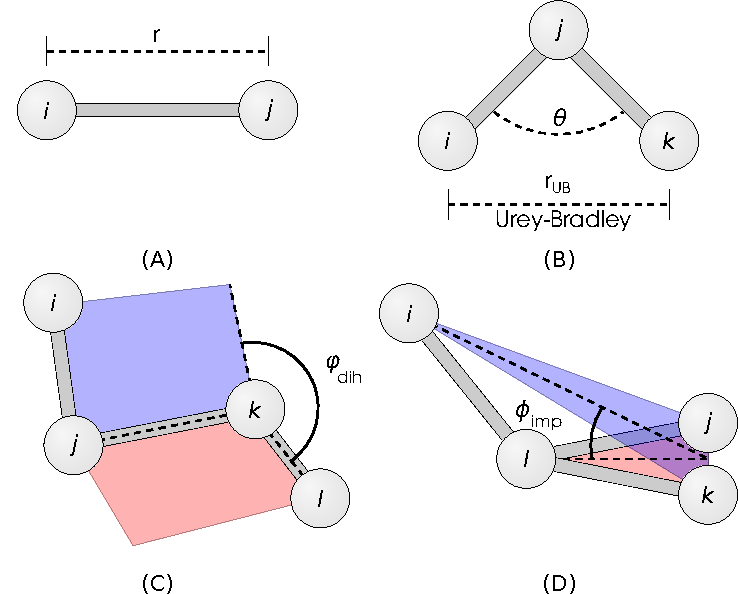
\includegraphics[width=10cm]{figures/bonded_interactions.pdf}
	\end{center}
	\captionsetup{singlelinecheck = false, justification=raggedright}
	\caption[The Bonded Interactions Calculated In Classical Forcefields]{\textbf{The Bonded Interactions Approximated In Classical Forcefields.}}{
		(A) The energy of Bond Stretching is approximated as a harmonic oscillator with respect to their separation $r$. (B) Angles between neighbouring covalently bonded atoms are also approximated as a harmonic oscillator with respect to the angle $\theta$. In some forcefields such as CHARMM there is a correction term for these angular interactions known as Urey Bradley forces. This is calculated using the separation between the non-bonded atoms $i$-$k$ in the triplet with the parameter $r_{UB}$. (C) The dihedral angle between four atoms is calculated by constructing two planes. Each plane is constructed to contains three of the four atoms in the set. One plane encompasses atoms i, j and k here  colored in blue and the other plane contains the j, k and l atoms colored in red. The dihedral angle is then calculated by taking the angle between these two planes along the line they intersect, the line formed by the j-k bond. (D) The improper dihedral angles are again calculated with the use of two planes. Containing i, j and k and j, k and l respectively. The difference is that this parameter parametrises planarity of a molecular configuration rather than the flexibility of torsion angles.
	}
	\label{charmm_bonded}
\end{figure}


In classical forcefields the non-bonded interactions are expressed using the Couloumb's law because the partial charges assigned to each atom and the Lennard-Jones potential to approximate the interactions arising from both Pauli exclusion and Van Der Walls Interactions.


\begin{equation}\label{nonbonded_eqs}
	\begin{aligned}
		U_{non-bonded} = \underbrace{\sum_{i>j} \epsilon_{ij} \Big( \Big(\frac{\sigma_{ij}}{r_{ij}}\Big)^{12} - \Big(\frac{\sigma_{ij}}{r_{ij}}\Big)^{6} \Big)}_{U_{Lennard-Jones}} - \underbrace{\sum_{i>j} \frac{q_i q_j } {r_{ij}}}_{U_{coloumb}}
	\end{aligned}
\end{equation}


The $\sigma$ parameter denotes the location of the local minima in the Lennard-Jones potential. This is the optimum distance that two atoms will rest against each other in the absence of other effects. The $\epsilon$ parameter denotes the depth of the potential well, or how stable the two atoms will be in the minimum energy configuration. This is very important for certain physical parameters such as osmotic pressure  \cite{Yoo2018}

Conversely, the partial charges in a system have the greatest influence on the solvation energy.

By focussing on these two physical parameters we can isolate and improve the non-bonded parameters.

\begin{figure}
	\begin{center}
	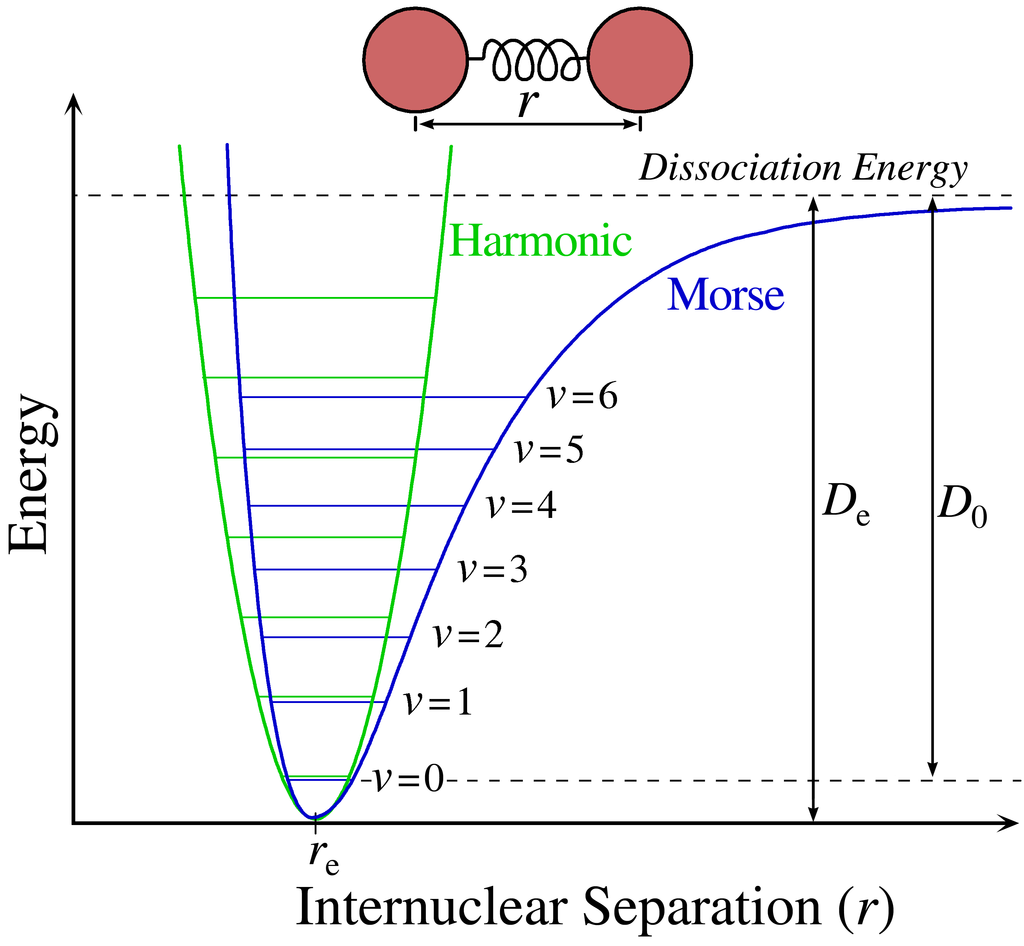
\includegraphics[width=7cm]{figures/Morse-Potential.png}
	\end{center}
	\captionsetup{singlelinecheck = false, justification=raggedright}
	\caption[The Morse Potential Compared to a Harmonic Potential] {\textbf{The Morse Potential Compared to a Harmonic Potential}}{
		The Morse potential was formulated to approximate the potential the potential energy surface of the separation of covalent bonds (blue). At low temperatures (the ground state, v=0) like those found in classical MD there is good agreement between the Morse potential and the harmonic oscillator (green). Credit Mark Somoza 2006. 
}
	\label{morse_potential}
\end{figure}

\subsection{Philosophy of Different Molecular Mechanics forcefields.}
At the time of writing, the four popular forcefields for the simulation of biomolecules are: AMBER, CHARMM, GROMOS and OPLS. Each of these have a slightly different philosophy in their formulation. They may be bottom up, as in the case of AMBER and CHARMM or top down, in the case of GROMOS and OPLS. Bottom up forcefields take the results from quantum \textit{ab initio} calculations and approximate them with the functional form mentioned above. Conversely, top down forcefields take experimental measurable such as Osmotic pressure, solvation energy. This philosophy is closest to physics 

\subsection{The Process of Preparing a Simulation}
The process of taking a molecular structure and putting it in a cellular environment to simulate it at physiological temperatures is both an art and a science. It's a science because a biophysicist must be aware of the many tricks that structural biologists use to image a macromolecular complex. But it's an art because accounting for those tricks and modifications is rarely straight forward. How do you build a missing loop? What charge state is an amino acid most likely to take during the physiological context.

\subsection{Controlling the Temperature and Pressure in a Simulation}

\subsection{Periodic Boundaries to Simulate a Realistic System Size}


\subsection{Short Comings of Classical MD}
The short comings of classical molecular dynamics fall into two classes whose solutions stand opposed to one another. These are the accuracy of the chemical forcefields outlined above and the inability of modern computers to deliver enough samples of the energy landscape to collect sufficient statistics for rigorous conclusions. The issue is that, as the above physical formulation might indicate. The more accurate the forcefields, the more computationally expensive. And so the solutions to the two are constantly in tension with one another. In the next section we will explore the current efforts to bring solutions.

\subsubsection{The Problem with Forcefields}
These approximations are not without a cost to accuracy. In certain situations, many of which are biologically relevant, it has been shown that quantum effects such as polarisation play an important role in the dynamics of the system. This has been demonstrated in the literature for Gramicidin where polarisable forcefields are able to more accurately reproduce the experimental results of current.

The other context where polarisation is important to consider are on divalent ions. Here, the solvation energy is underestimated due to the consistent lack of polarisation, making investigations of these biologically important chemical species difficult.

However, for most situations, particularly those involving bulk water and protein motions Molecular Dynamics is proving to be an invaluable tool for investigating the properties of biological systems CITATION NEEDED. Sadly, it should be kept in mind that classical MD is not able to simulate any chemistry such as forming and breaking or the change a change in profanation state. Such interactions require considerations of Quantum Mechanics which are computationally expensive.

There are several efforts to correct address some of the above issues. These include the inclusion of the effects of polarisation, the most popular methods at the moment being adding a massless drude oscillator as an extra bead to most(?) atoms as in the CHARMM drude forcefields, championed by the Mackerell lab and the use of forcefields such as AMOEBA which explicitly calculate the dipole and quadrupole moments of each atom. These both substantially increase computational cost but have displayed much better agreement with experiments in biological systems where classical forcefields have been shown to fail \cite{ngo2021}. 

Ultimately, the functional form in equation \ref{CHARMM} does not have sufficient degrees of freedom to address all possible chemical contexts  and so careful consideration must always be given to whether the forcefield is being used in a faithful way to what it was intended to simulate. So long as the user is aware of the situations where classical forcefields fall short they can be a powerful tool for the study of molecular systems.

\subsubsection{The Problem with Sampling}

To physicists the sampling is the more intuitive. Collecting sufficient statistics about the system of interest is difficult and comes at both a computational and human cost. Even though computers have sped up exponentially for the last 50 years we are still orders of magnitude from being able to reach the time scales of many biological processes. As is we struggle to sample the time scales of diffusion through an ion channel, despite the problem standing for decades. 

The slow time step demanded in classical MD due to the fast motions of certain atomic groups such as hydrogen is fundamentally at odds with the time scales of many important biological processes such as drug binding or protein folding which occur on the time scale of  milliseconds or seconds. 

Methods are now emerging which intelligently drive the simulation toward regions unexplored in the collective variable space by unbiased simulations. For some time the field has used steered methods or adaptive sampling methods such as Umbrella Sampling or Metadynamics to drive the simulation toward sections of the energy landscape which are under sampled. These methods universally rely on a choice of collective variable which closely corresponds to a slow degree of freedom. Such a choice is not usually simple. In the case of ion channels one may rationally choose the placement of the ion along the conduction pathway as the collective variable but the choice is less obvious in the case of more global conformational changes.

The advances we are seeing at the moment which I find exciting are the use of machine learning methods to tease out these degrees of freedom in order toaccelerate them with already established free energy methods. These have the potential to uncover new drug binding pockets and revolutionise our understanding of biomolecular systems. 


\subsection{Accelerating Simulations with Virtual Site Topologies}
The discrete time step, $\Delta t$ in equation \ref{verlet}, is one of the most important determinants in the performance of the simulation. We would like $\Delta t$ to be as large as possible, so that the minimum number of calculations are made to sample the desired time scale, which usually runs to nanoseconds or milliseconds.  

Due to Nyquist's theorem the $\Delta t$ parameter must be less than half the speed of the fastest degree of freedom in the system CITATION NEEDED. In the case of biomolecular systems we are challenged by the fact that they are so hydrogen-rich. Since hydrogen is so light, its motion is much faster compared to the other molecular motions involving heavier, slower moving atoms. Its correlation time is on the order of 1 femtosecond, in classical simulations we are able to get away with using 2 femtoseonds by enforcing a rigid hydrogen bond length, i.e interpolating its position backward from the 2 fs timestep.  

However, there are more involved strategies to account for these effects. Hydrogen Mass repartitioning and multiple time stepping have become popular but we will discuss Virtual Sites in detail as they were used for some simulations in this thesis.  

\begin{table}
	\begin{center}   
		\begin{tabular}{ |c|c|c|}
			\hline
			Motion & Timescale \\
			\hline
			Covalent Bond-stretching & $1-2\times10^{-15}\text{s}$ \\
			Covalent Bond-angle bending & $5-10\times10^{-15}$s \\ 
			Sidechain  Motions & $1 \times10 ^{-12}\text{s}-1\times{10^-6}s$ \\
			Rigid Body Motions (depending on size of body) & $1 \times10 ^{-9}\text{s}-1s$ \\
			Ion Conduction & $1\times10^{-9}\text{s}-10^{-6}$ \\
			Protein Conformational Changes & $1\times10^{-9}\text{s}-10^{-3}$ \\
			Alpha Helix Formation & $1\times10^{-9}\text{s}-10^{-6}$ \\
			Beta Sheet Formation & $1\times10^{-6}\text{s}-10^{-3}$ \\
			Protein Folding & $1\times10^{-6}\text{s}-10\text{s}$ \\
			\hline
		\end{tabular}
\end{center}
%\begin{tabular} { |c|c|c| } 
%	\hline
%	%\label{atomic_motions_speed}
%	System Description & Fastest Degree of Freedom & Characteristic Timescale \\ 
%	\hline
%	Uncoupled Atoms  & Atom Translation & 10 fs  \\ 
%	Rigid Molecules & Rigid Body Rotation & 5 fs \\  
%	Flex. Molecule with Rigid Bonds & Bond Angle Vibrations & 2 fs  \\ 
%	 Flex. Molecule with Flex. Bonds & Bond Stretching Vibrations & 1 fs  \\ 
%	\hline
%\end{tabular}
	\captionsetup{singlelinecheck = false, justification=raggedright}
	\caption[Timescales of Motions in a Molecular System]{\textbf{Timescales of Motions in a Molecular System}} {The time step of a simulation must be small enough to capture the motions in the fastest degree of freedom. In hydrogen-rich biomolecular systems the bottle neck can be found in the fast bond vibrations in lighter atoms. This stands in tension with the phenomena we are interested in on longer timescales such as protein folding. Sources: \cite{schlick2010}\cite{brooks1988}\cite{flood2019}\cite{werner2012}}
\end{table}

As you can see in table \ref{atomic_motions_speed} the fastest motion in molecular systems is dictated by the translation of hydrogen atoms. Virtual site topologies aim to remove the requirement for calculating these motions every time step by instead interpolating the positions of hydrogen atoms from the positions of surrounding heavy atoms. This follows from the 3600cm$^{-1}$ peak in the resonance infrared resonance spectrum of biomolecules corresponding to the bond stretching oscillation of the H-O bond. \cite{schlick2010} Setting the time step of simluations to 1/10th of this period gives sufficient gives the Verlet integrator sufficient resolution to capture the motion and maintain the stability of the energy function.

\section{Free Energy Calculations: Making Simluations More Useful}
The above work sets out how to perform unbiased MD simulations. These are powerful tools but as mentioned in section \nameref{sampling_problem} if one only relies on unbiased simulations they will quickly exceed the available computer power. So we must be clever in how we direct our available resources. This means intelligently sampling sections of the molecular phase space which are of interest to us physically but are not reached in our unbiased simulations. A technique that is used extensively throughout this thesis is the addition of a biased potential to the molecular potential $U_{MM}$ calculated for the purposes of unbiased simulations. This will drive the simulation to regions of interest. 

\begin{equation}
U_{FEC}  = U_{MM} + U_{biased} (\xi)
\end{equation}

Note how the $U_{biased}$ term is explicitly dependent on a parameter $\xi$. This parameter is known by many names, an order parameter, a collective variable or a reaction coordinate. Each of these names 

\subsection{Umbrella Sampling}

\subsubsection{Weighted Histogram Average Method}

\subsection{Metadynamics}


%=======================================================================================%
\chapter{Review of the Molecular Cause of Cystic Fibrosis and Its Treatment}
\label{chap:cftr_review}
\chapquote{Because of what's inside me; Because of my genes;-Bob Flanagan, "Why."}{}
\newpage
%Authors note:
% We begin with a breif overview of the disease Cystic Fibrosis as it is the main motiation for this project. A horrendous disease for which we will soon find a cure.
% The purpose of this chapter is to present an overview of CFTR's structure and mechanism of action as discovered by a combination of structural and physiological studies. In addition to the actions of CFTR modulators.
\section{Clinical outcomes of Cystic Fibrosis}
Cystic Fibrosis (CF) is the most common fatal genetic condition in Caucasian populations. 165 000 people are afflicted globally. Even with decades of research there is no known cure for CF. With the average life expectancy of patients falling below 50 even in countries with developed health care systems such as the USA and Australia\cite{}\cite{}. The cause is from a build up of salts inside epithelial cells. This causes the surface of the epithelium to dehydrate. When dehydrated the cilia on the epithelium collapse leaving them unable to clear the mucus that naturally lines the airway\cite{boucher2007}. The dehydration mentioned earlier causes the mucus to thicken. This buildup has two pathogenic functions. Firstly it inhibits the normal function of the organ, as mucus fills ducts that would normally pass nutrients in the pancreas or absorb gasses in the lungs. Secondly, the stationary mucus allows bacterial infection, this can further degrade lung function and remains one of the most troublesome chronic complications in CF patients. 

Much of the clinical research into CF has been managing the movement of this mucus and the populations of bacterium in it. Patients require hours of physical therapy each day to help clear this mucus since their lungs are unable to. They must also inhale saline solutions in order to counteract the osmotic pressure in their epithelium. This helps draw more moisture out of the epithelial cells to allow the cilia to move. 

CF patients struggle to intake nutrients due to the build up of mucus in the ducts of their pancreas and large intestines. This leads to CF related diabetes which afflicts roughly half of adults with CF \cite{Kayani2018}. Patients with CF related diabetes are often administered enzymes and must adhere to a specific diet. 

\begin{figure}
	\label{CF_life_expectancy}
	\begin{center}
	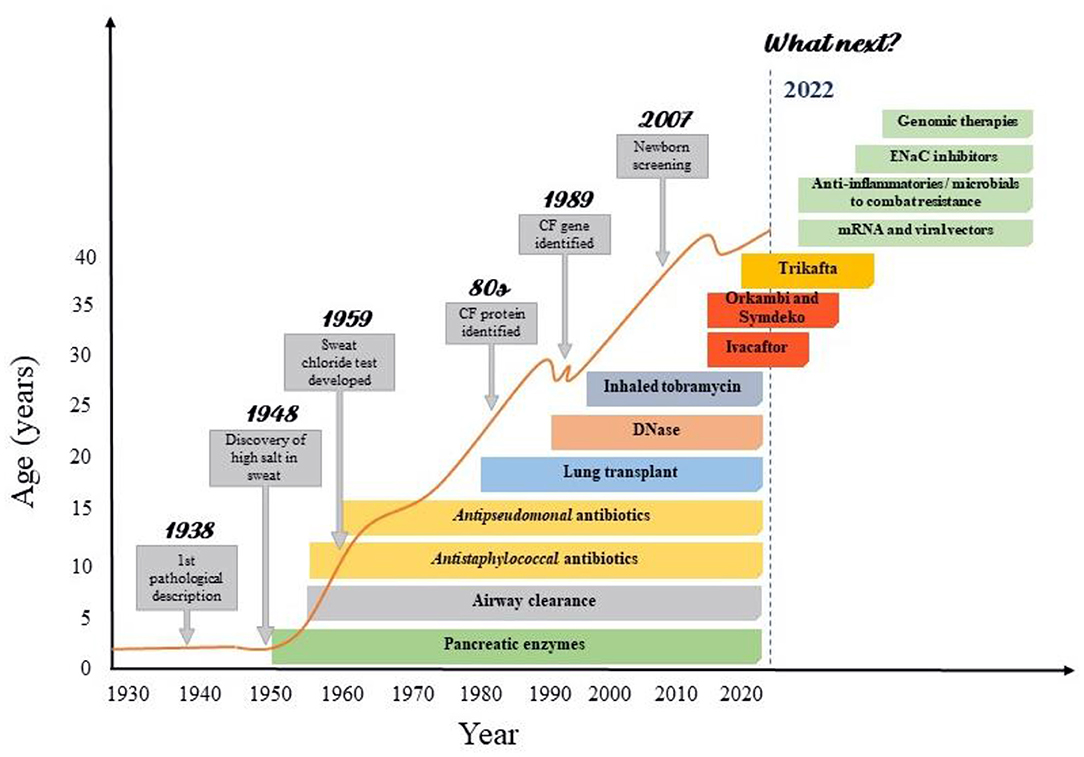
\includegraphics[width=0.6\textwidth]{figures/CF_life_expectancy.png}
	\end{center}
	\captionsetup{singlelinecheck = false, justification=raggedright}
	\caption[CF Clinical Progress] {\textbf{CF Clinical Progress}}{Life expectancy of CF patients correlates highly with translational research. Source \cite{garcia2022}} 
\end{figure}

\section{CFTR Structure}

\begin{figure}
	\begin{center}
	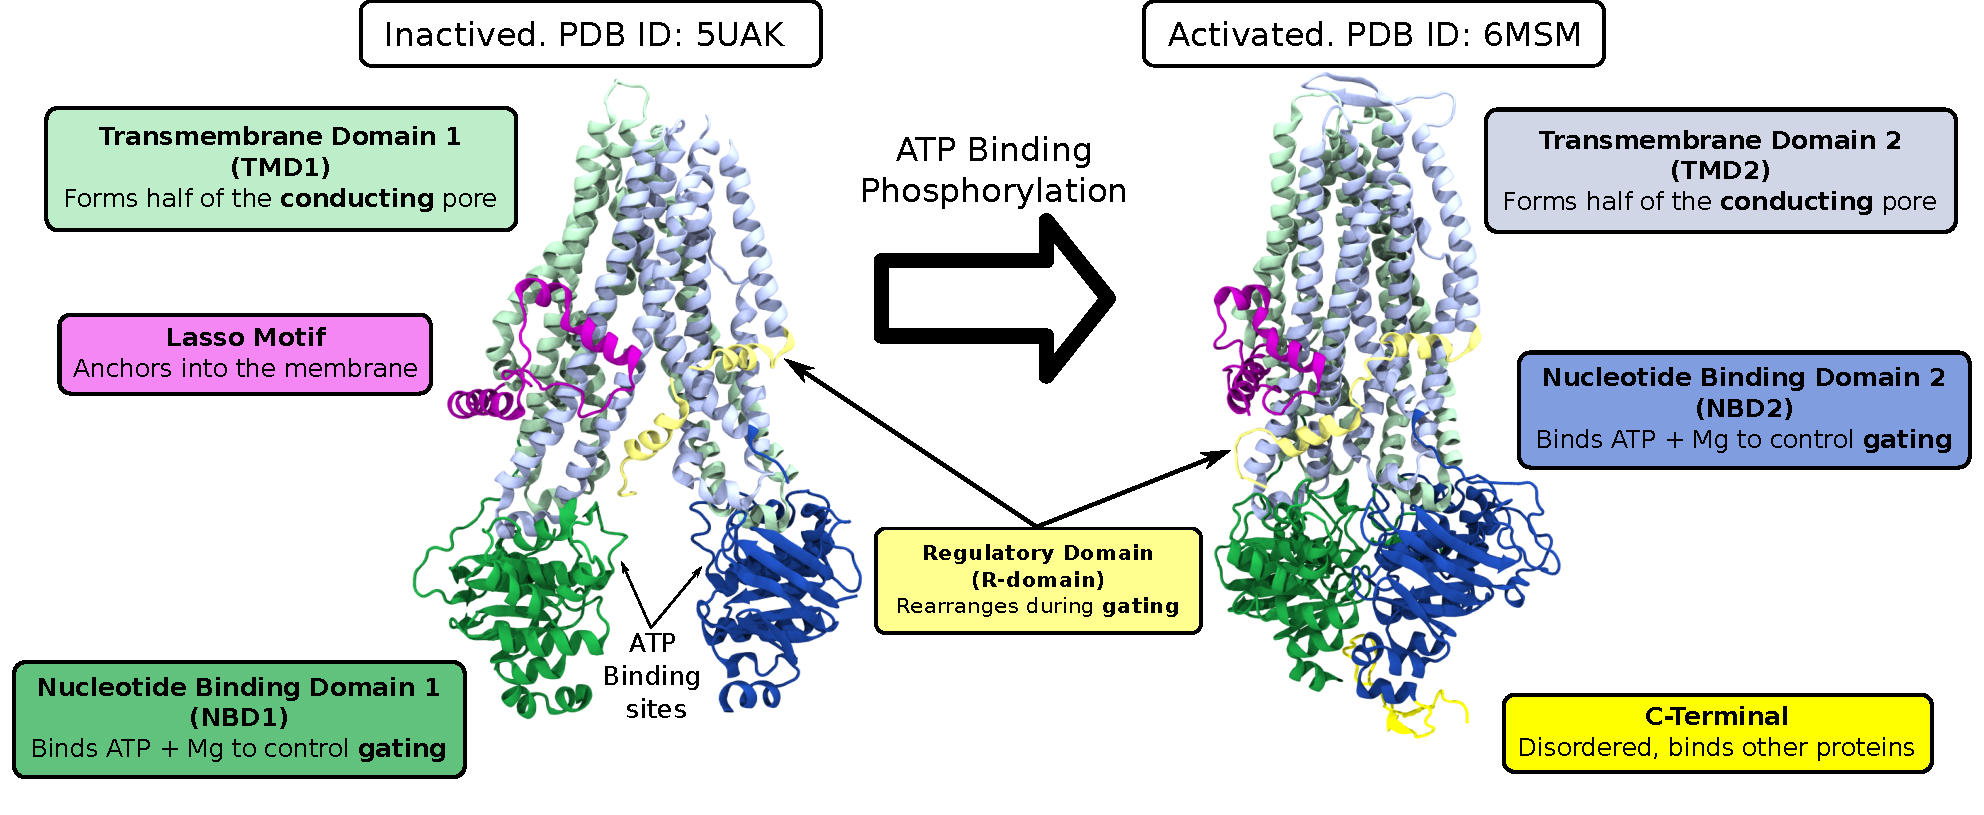
\includegraphics[width=\textwidth]{figures/CFTR_structure.pdf}
	\end{center}
	\label{CFTR_structure_domains}
	\captionsetup{singlelinecheck = false, justification=raggedright}
	\caption[CFTR Structure] {\textbf{CFTR Structure}}{There are currently two resolved human structures. The inactivated state is neither phosphorylated nor bound to ATP. Observe how the NBDs are far apart and the TMDs are not parallel, forcing a constriction which does not allow the passage of ions. By contrast, the activated structure is abound to ATP at both sites, bringing the TMDs into a parallel configuration where they form a pore. There are unresolved questions as to whether CFTR may conduct chloride in this conformation which we will analyse in chapter \ref{chap:opening}.} 
\end{figure}
CFTR is composed of one chain with pseudo-symmetric structure, the protein is well organised into 7 domains \ref{CFTR_structure_domains}. In the order of their primary structure they are: 
\begin{enumerate}
	\item The Lasso motif (AA 1-68). Anchors into the membrane and serves as an interaction hub with protein partners such as syntaxin and filamin which are important in cellular trafficking \cite{cormet-boyaka2002}\cite{naren1998}\cite{thelin2007} as well as WNK1 which plays a role in bicarbonate selectivity \cite{kim2019}.
	\item Transmembrane Domain 1 (TMD1 AA 69-376). This domain forms half of the chloride conducting pore and importantly, in the activated human structure 6MSM forms the extracellular  pore for anion permeation\cite{}.
	\item Nucleotide Binding Domain 1 (NBD1 AA 377-629). One of the ATP binding sites, this domain has a dense concentration of disease causing mutations, including the most common mutation $\Delta F508$ \cite{thehospitalforsickchildren2020}.
	\item Regulatory Domain (R-domain AA 630-855). A disordered domain containing up to 11 phosphorylation sites\cite{mihalyi2020}. In the inactivated conformation a helical segment of this domain wedges between the TMDs. Upon binding of PKA and phosphorylation the wedge relocates to a location just below the R-domain. The identity of this wedge is analysed in detail in chapter \ref{chap:I37R}. The kinetics of this domain is important to the overall function of CFTR. 
	\item Transmembrane Domain 2 (TMD2 AA 856-1168). This domain forms the other half of the chloride conducting pore. There is ongoing controversy over the structure and function of TM8 the function of CFTR \cite{hegedus2022}\cite{liu2019}.
	\item Nucleotide Binding Domain 2 (NBD2 AA 1169 - 1450). Home to the conserved Q-loop, which plays an important role in the binding of ATP in ABC transporters \cite{ivey2020}\cite{zolnerciks2014}\cite{dong2015}.
	\item C-terminus (NBD2 AA 1451 - 1480). 
\end{enumerate}
Transmembrane Domain 1 (TMD1) which forms half of the pore. Nucleotide Binding Domain 1 (NBD1) which binds ATP when the channel is in the open state. The Regulatory domain (R-domain) which, when phosphorylated allows the channel to open. Transmembrane domain 2 (TMD2) which forms the other half of the ion conducting pore. Nucleotide Binding Domain 2 

CFTR belongs to a super family of proteins known as ATP Binding Cassette Transporters,  many of these proteins perform active transport across cell membranes. The substrates they transport can vary, including lipids and drug molecules. Proteins in this family share a common motif known as Nucleotide Binding Domains (NBDs). These domains act as ATPases, accelerating the hydrolysis of ATP. The energy from hydrolysis is then transferred into the protein in order for it to pump its substrate against a concentration gradient. 

\section{CFTR is a Unique ABC Transporter}

\begin{figure}
	\label{ABC_diversity}
	\begin{center}
	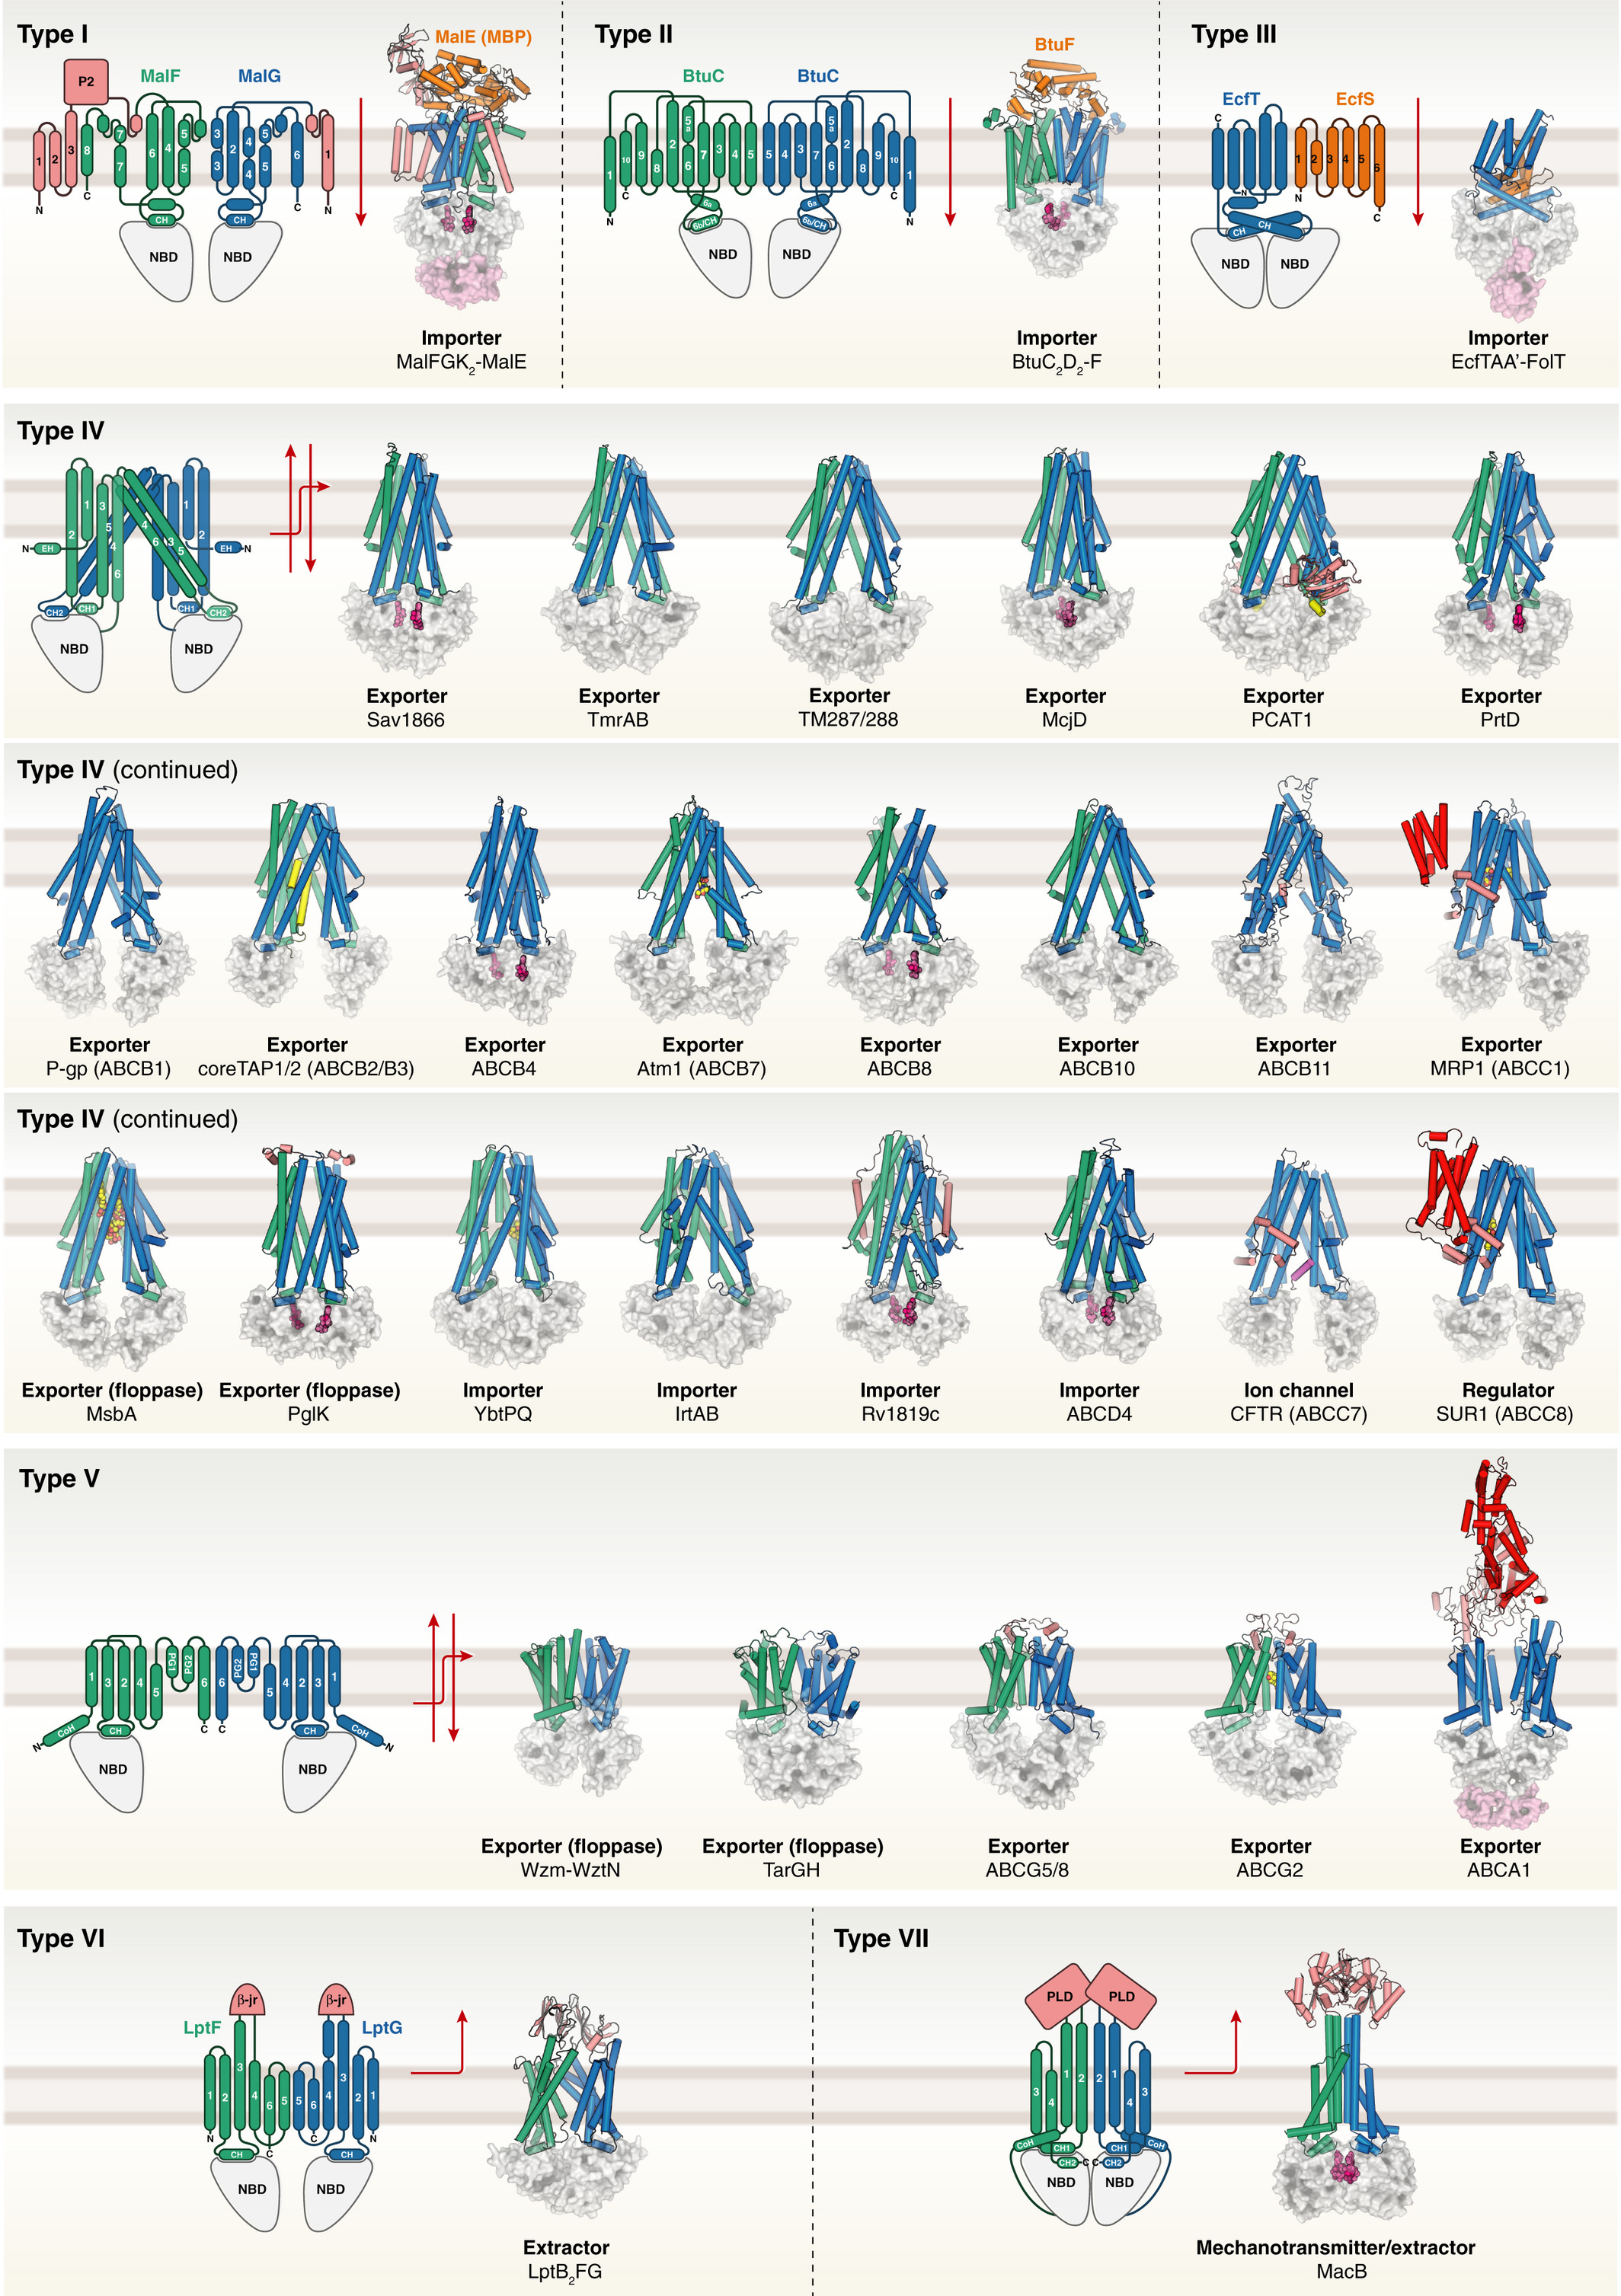
\includegraphics[width=\textwidth]{figures/ABC_classification.jpg}
	\end{center}
	\captionsetup{singlelinecheck = false, justification=raggedright}
	\caption[CFTR Structure] {\textbf{CFTR Structure}}{The structural diversity of ABC transporters. Structures are classified based on the organisation of their TMDs source \cite{thomas2020}.} 
\end{figure}
ATP-Binding Cassette (ABC) transporters are an intriguing super family of proteins. On the whole, they transport substrates by using a combination of phosphorylation energy from ATP hydrolysis. These can be diverse substrates such as lipids or small molecules. Their structural diversity can be seen in figure \ref{ABC_diversity} reflecting their array of functions. 

CFTR is unique, as it is not a transporter, but rather an anion \textit{channel}. The kinetic energy of the ATP is not used to translocate substrate across the membrane but rather simply used in the regulation of the gating cycle. Chloride, bicarbonate and other anions are able to \textit{passively} diffuse through the channel. This evolutionary misappropriation of a transporter to a "leaky channel" is perhaps the reason so many mutations can create a non-functional protein \cite{linsdell2018}.

\section{CFTR classification and structure}

The primary cause of the disease Cystic Fibrosis (CF) is the malfunction of a chloride channel, the Cystic Fibrosis Transmembrane Conductance Regulator (CFTR). This ion channel is a member of the ABCC subfamily of ABC transporters, designated ABCC7. This channel is unique amongst this family because it is not generally considered an active transporter but something of a low conductivity channel or a "weak pump"\cite{linsdell2018}.

CFTR is distinguished by a regulatory region known as the R-domain (residues 645-845) which links NBD1 to TMD2. This region acts to lock the channel in the closed state by wedging itself between the TMDs and dislodging when any one of 3 sites are phosphorylated \cite{mihalyi2020}. In experimentally determined structures of human CFTR the secondary structure of a section of the R-domain but not at high enough resolution to determine the identity of individual side chains \cite{zhang2018}\cite{zhang2016}. Further secondary structure information can be found through experiments with NMR \cite{Baker2007}.

Previous computational studies of CFTR have been used homology models based on the phosphorylated zebra fish protein PDBID:5W81 \cite{zhang2017a}. These have yielded interesting results but the sequence similarity between human and zebra fish CFTR is only 55\% \cite{}. For a protein structure where a single amino acid mutation leads to malfunction, more precision can only help. Additionally, the activity of CFTR modulators is not conserved in mutant zCFTR possibly because it has different kinetics to the human channel \cite{}. In order to do precision medicine we need precision structures. 

An open state of the channel has been proposed by combining both the zebra fish homology model and the fully outward facing conformer of a bacterial ABC transporter Sav1866 \cite{Hoffmann2018}. Although this model has several characteristics expected of the open channel, such as the critical R352-D993 salt bridge, it lacks a salt bridge between R104-E116. In experiments, these residues could be replaced by cysteines and the channel would still function. However, when reducing agents were added to the system the channel lost its ability to open fully. This indicates that in the oxidised environment the C104-C116 cysteines formed a disulfide bridge but its breaking upon exposure to reducing agents caused a loss of function in the channel. This indicates that in the WT channel R104-E116 form a stable salt bridge. 

This salt bridge is clearly visible in the recent cryo-EM structure of ATP-bound human CFTR \cite{zhang2018}.

\section{The Gating Cycle}
The conformational transition from inactive to active differs significantly in CFTR compared to other ABC transporters. The NBDs are largely similar to other to those found in other ABC transporters, they dimerise in what is termed a head to tail configuration so both subunits contact both bound ATP molecules \cite{} See FIGURE. Residue E1371 allows nucleophilic attack on the $\gamma$ phosphate of the ATP bound to Walker B \cite{Stratford2007}. This provides a "kick" to provide the kinetic energy for the opening of the channel CITATION NEEDED. 

\section{Classes of Misfunction to CFTR}
The 360 disease causing mutations to CFTR have been classified into 6 common classes based on the nature of the CF they cause, their reaction to CFTR modulators, and results \textit{in vitro} assays. Ultimately I aim to show that at the atomic level these classes of mutations are less meaningful and as patient specific theratyping evolves these classes will become less relevant, serving as illustrative tools only to communicate at a higher level what is going wrong with the CFTR protein. The canonical classification is as follows:
\begin{itemize}
	\item \textbf{Class I} No functional protein. Under these mutations no protein is transcribed due to either problems with the transcription of mRNA or a premature stop codon truncating protein synthesis early, meaning the resulting peptide is missing key domains. 
	\item \textbf{Class II} Folding defect. These mutations cause the translated peptide to misfold into the incorrect tertiary structure. This can inhibit the protein's journey as it is trafficked to the cell membrane, its function while once it is there or its functional life time at the surface. 
	\item \textbf{Class III} Impaired Gating. Here the mutation inhibits the ability of the protein to transition from the closed to the open state. 
	\item \textbf{Class IV} Decreased Conductance. These mutations cause a barrier in the energy landscape of the CFTR chloride conductance pathway.
	\item \textbf{Class V} Less Protein Expressed.  
	\item \textbf{Class VI} Decreased Lifetime

\end{itemize}

Although useful, in reality this paradigm struggles to reflect the fact that a mutation can belong to multiple categories to different levels due to different modes of pathogenesis. Through our molecular simulations we can see that in reality CFTR modulators are capable of treating several different mutations with very different molecular fingerprints. We will break down this paradigm into more molecular detail in chapter \ref{chap:outlook_review}

FIGURE demonstrates how each of the canonical classes at the molecular level is broken down into many sub classes and a mutation might belong to one of many of these subclasses. Structural biology paradigms and \textit{in silico} modelling can help classify mutations into these different classes. In combination with wet lab assays we can understand which classes of these molecular defects are most effectively treated with specific drug regimens. Our computational microscope is helping choose treatments for patients at the atomic level. 

\section{CFTR Modulators}
Since CF is caused by malfunctions of the channel it makes sense to pursue CFTR as a drug target. Through high throughput \textit{in vitro} screening several (GET NUMBER) compounds have been developed that aim to rescue the function of CFTR. These fall into two classes. Correctors, which aid CFTR to fold into the correct state and potentiators which help the channel reach the fully open state once it has already folded correctly. Emerging evidence suggests that specific genetic defects may be optimally rescued by specific combinations and doses of both correctors and potentiators compounds. Recently, cryo-EM structures of these compounds in their bound state have been released. In addition to several \textit {in vitro} biophysical experiments to determine the precise mechanism of action and binding site of these compounds.

\subsection{Correctors}
The mechanism of action for corrector compounds appears to be to bind to to a pocket between TMH1 and TMH3. Circular dichromism and fluorescence experiments found that an isolated construct of TMH3 and TMH4 were more likely to fold correctly in the presence of corrector compounds. Later cryo-EM structures discovered high resolution electron density in the pocket in the shape of the drug compounds \cite{fiedorczuk2022}. 

In combination this is strong evidence for the precise mechanism of action for corrector compounds. Further work will aid in the creation of new compounds to refine our exploitation of this mechanism.

Mention that there are some interactions between correctors and NBD1.

\subsection{Potentiators}
There is more uncertainty surrounding the mechanism of potentiators drugs. Experiments clearly demonstrate that they act directly on CFTR in order to increase the likelihood that it occupies the open state. They bind to the protein with picomolar affinity. There are are cryo-EM structures which show the drugs bound to the TM8 hinge region \cite{}. \textit {In vitro} experiments suggest at least two membrane facing binding pockets due to the drugs extreme hydrophobicity\cite{}. The location of this second binding site is unknown. The difficulties arise with mutagenesis experiments. The dose-response curves in several studies show that when various sites are mutated the activity of the drug is lowered. This indicates additional binding sites not yet well defined. 

GLPG1837 has not been approved in a clinical setting. \textit {in vitro} experiments suggest that it is more efficacious even though it has lower affinity for CFTR binding (CITATION NEEDED). This would indicate that the highest affinity binding pocket does not produce the greatest modulation. More work is needed to resolve the mechanism which results in the clinical effectiveness of these drugs.  

These drugs are clinically efficacious \cite{VanGoor2014} on several mutants with some curious exceptions like N1303K. I suggest the following mechanism for their action. I suspect a similar analogy exists for the action of the correctors. WT-CFTR exhibits a natural landscape with kinetic barriers in the transition between the closed and open states. A gating class mutation to CFTR will introduce a kinetic barrier in the pathway of this conformational transition. What these drugs do is reduce a barrier in the existing conformational landscape of CFTR. This compensates for the barriers introduced by the mutation. 

This provides a rationale for why it appears possible for diverse range of molecular defects to be treatable by these small molecules. In our work we've found that the atomic nature of the defects introduced by each mutation varies widely, what is interesting is that experiments in \textit{ex vivo} models have shown that these drugs treat a variety of different defects. The classification of classes of defect is outdated, really there are as many classes as there are mutations.


\subsection {Anion Selectivity}
CFTR is weakly selective for specific anions. F337 is the most important amino acid for selectivity. Bicarbonate (HCO$_3^-$ is known to have roughly 26\% the permeability of chloride through the channel. Note that Fluoride has even higher conductance through CFTR, likely due to its small size and high solvation energy (does this indicate hydrated conductance?). WNK1 is known to influence the selectivity of the channel https://www.ncbi.nlm.nih.gov/pmc/articles/PMC6889609/. The permeation of bicarbonate is very important physiologically because if a mutation permeates bicarbonate it means there is a high likelihood the patient will be pancreatic sufficient. 

Compared to cation channels like Gramicidin and KcsA, CFTR is only weakly selective, permeating a large set of annions with varying radii and geometries. Supposedly it is more permeant to lyotropic (low solvation energy annions) rather than cosmotropic anions (high solvation energy annions) indicating that dehydration of the anion is likely during conductance (CITATION NEEDED). The radius of hydrated chloride ions is 1.7A\cite{yang2002} so even with this larger pore partial dehydration must take place. 

\section{Addressing Controversies Surrounding the Structure of CFTR}
The most recent structure of human CFTR in a phosphorylated environment has some interesting features which have lead to some controversies in the literature. After spending significant time researching them I have conducted an extensive literature review in order to learn more about of these concerns. The released structure of activated, human CFTR has two features that have caused some in the CF field to suggest issues with this structure. Firstly, this structure is not sufficiently open to conduct chloride ions. Chloride ions have a diameter of 1.7$\AA$ while the structure has a constriction of 1.1$\AA$\cite{Zhang2018}. So, there must be some level of conformational changes, even if chloride were to move through the channel completely dehydrated. This becomes even more of an issue when considers the experimental evidence where much larger anionic species such as bicarbonate and glutathione were shown to permeate through the channel\cite{kogan2003}. This suggests that there is a much larger conformation which has not been observed experimentally or in simulations. This was the motivation for chapter \ref{chap:opening} of this thesis. Some studies have been performed in order to study the possible permeation paths of chloride but they have not addressed the pressing question of how larger ions might permeate the channel. Bicarbonate in particular is of great physiological importance as there is a high correlation between the channel's ability to permeate bicarbonate and the pancreatic sufficiency of a patient carrying the mutation. In light of this, structural knowledge of a fully open conformation of CFTR is critical to a personalised approach to the treatment of CFTR.

The second and harder to resolve controversy concern the role of TM8. This transmembrane helix has an unusual bend in the middle of the plasma membrane. This is not something seen before in ABC transporters of this type. So it has led to some open questions as to how this bend might contribute to the function of the channel \textit{or} how it might be an artifact of the imaging process. For the former case, the structural biologists in the Chen lab proposed a mechanism whereby the upper hinge of TM8 swings 55$^o$ during the transition to the open state. This mechanism would give justification of the pathogenesis of certain mutaions such as L927P. 

The arguments for the bend in the helix appear to be unphysical. In cryoEM structures, we can observe that the bent conformation is stabilised by salt bridges R347-D924 and E873-R933. The former bond has been well studied experimentally and was expected in the 3d structure. Additionally, all hydrogen bonds along the in the bent helix are . Been observed to be stable in MD \cite{corradi2018} .  is energetically stable.

However, there are still some unanswered questions for the discrepancy between the solved human and solved chicken structures. Certain salt bridges are not present in the latter structure and so single channel electrophysiology experiments may be able to resolve these issues. For example, in 6MSM, the human structure of CFTR there is a salt bridge between amino acids 933 and D873 which is not present in the chCFTR structures. This bond is also present in the zCFTR structure 5W81. If a charge swapped mutant such as R933E/E873R restores WT-like gating behaviour to the channel it would be  strong evidence for the unwound conformation of TM8. 

The two proposed conformations also have vastly different ion permeation pathways, and so blockers engineered to target one conformatoin over the other would also go a long way to answering these questions. The available evidence strongly favors the R334 pathway between TM1 and TM6. Such as experiments to  demonstrate the blockage of current with zinc have shown that mutations to R334 strongly suggest that chloride permeates along this route. Additionally, trhere are several disease causing mutations in the region surrounding R334, such as R334W, R117H, E116K, D110H, I336K\cite{cftr2}. This permeation route also explains the rationale behind the gain of function mutation F337A \cite{}. Determining which model is correct has wide implications for creating the next generation of mutation targeted potentiator class drugs.

A study assessing the accuracy of Alphafold's predictions of transmembrane protein structures found an intersting result. When alphafold made predictions that involved the use of templates it predicts the unwound conformation of TM8. On the other hand, when templates are removed from alphafolds predictions it predicts a straight TM8 conformation, very similar to that found in chCFTR. The authors of this study suggested the reason for the discrepancy was due to the use of detergents in the deteremination of the structure of hCFTR. However, careful reading of cryo-EM literature reveals no examples where the use of detergents has resulted in such drastic conformational changes. One of the few examples where both detergents and native-like nanodisks were used to determine the structure of a protein are the determinations of the structure of TRPV1. These studies revealed no difference to the backbone helices but did suggest important information about the the importrance of different interactions with lipids. A lot of work has been performed in order to create detergents which reflect a native lipid environment and these are the species that were used in . 

The authors of the chCFTR paper suggested that the different expression systems used in the two studies could be the reason for the discrepancy between the two systems, due it their different post translational processing apparatus. Although both groups used mammalian cell lines the chCFTR paper used hamster? cells \cite{aleksandrov2015} and the Chen lab used HEK293S cells. The chicken structure underwent significant mutations in order to be locked open and crystallised. The regulatory insertion was deleted, Many hydrophobic amino acids were introduced into NBD1 in order to aid in the purification of the protein. 

Figure \ref{} shows the large diversity of structures in type IV ABC transporters, many of which also exhibit bends within transmembrane helices\cite{thomas2020}. 
>>>>>>> dfa8ae7c815116d94d0aada27fa917fd6409538a

\section{Patient Derived Organoids}
The basic unit of living things are cells. In the medical field there is growing capability to discern the functioning of an individual patient's cells. In the field of Cystic Fibrosis Medical Research a recent breakthrough has been to take samples from the epithelium of patients with the disease and grow those samples into tissues which mimic the function of the entire organ\cite{depoel2020}. This is possible in the epithelium due to a population of adult stem cells which maintain the ability to differentiate into a variety of cell types (a property known as pluripotency). 

Adult stem cells in the epithelium are preferable because other sources of stem cells such as induced pluripotent stem cells (iPSCs) require complex, time consuming protocols to grow into fully developed organoids. 

In the case of CF this technology allows the construction of a scalable, patient specific platform where a patient's own tissues can be tested to determine the best treatment for them. These pre-clinical models will allow more patients in the heterogeneous set of disease causing mutations to access modulators. 

Forskolin Induced Swelling (FIS) assays have been used to characterise the patient specific response of a patient's organoids to a drug regimen \cite{dekkers2013}. 


One limitation of these organoid platforms is the lack of an inflammatory response since no immune cells are present in the tissue culture. 


%

%text

%%=======================================================================================%
\chapter{Mechanism of Ligand Binding in \GltPh}
\label{chap:bind}

ABSTRACT \newline

%%=======================================================================================%
\chapter{Escape of \Na\ from Na3 in \GltPh}
\label{chap:unbind}
ABSTRACT \newline
Glutamate/Aspartate transport through the mammalian excitatory amino acid transporters 
is coupled to the co-transport of three \Na, one \Hi\ and the counter-transport of \K. 
The archaeal homologue \GltPh\ is coupled to only the co-transport of three \Na. The 
first two \Na\ sites (Na1,Na2) were resolved from both the outward and inward the crystal 
structure. The third site (Na3) was determined through a combination of mutagenesis 
experiments and molecular dynamics simulations and later verified in the crystal structure 
of \GltTk. Previous studies using path-independent free energy methods have suggested 
unbinding of the last \Na\ from Na3 is the rate-limiting step. Here we use path-dependent 
methods to determine the path taken and energy required for \Na\ to leave the Na3 site to 
the bulk region to the bulk region. A detailed characterisation of structural changes of 
the binding pocket as \Na\ leaves the binding site are given. In addition, we estimate the 
release time of \Na\ using Smoluchowski mean-first-passage-time theory. Our observations 
of structural changes made along the path and estimated time of release are consistent 
with known experimental data. The results presented here indicate that the release of 
\Na\ in the third binding site is a slow process but not the rate-limiting step of the 
transport cycle. This investigation may shed light on the ligand release mechanism in 
the mammalian transporters.

\newpage
\section{Introduction}
The mammalian glutamate transporters, also known as the excitatory amino acid transporters 
(EAATs), are responsible for clearing excess glutamate released at the synapses. Disruption 
of EAATs can lead to increased concentrations of glutamate, causing excitotoxicity of receptors. 
Such effects have been associated with many pathological conditions, including Alzheimer's 
disease, cerebral ischemia and amyotrophic lateral sclerosis~\cite{Danbolt2001}. EAATs 
function by cycling between the extracellular and intracellular medium. In each cycle, EAATs 
bind and transport the substrate (Asp or Glu) across the membrane by coupling three \Na\ and 
one \Hi\ ions~\cite{Zerangue1996}. After the release of the ligands, one \K\ ion is 
counter-transported to complete the cycle. While much has been learned about the functional 
properties of glutamate transporters from mutagenesis experiments, a mechanistic understanding 
of the transport process was not possible in the absence of a crystal structure. 

The first crystal structure of aspartate/glutamate transporters was that of \GltPh\ from 
Pyrococcus horikoshii—an archaeal homologue of EAATs~\cite{Yernool2004}. In successive 
iterations of the \GltPh\ crystal structure, first, the binding sites for the substrate and two 
\Na\ ions (called Na1 and Na2) were resolved in the outward-facing (OF) state~\cite{Boudker2007}, 
followed by the determination of the inward-facing (IF)~\cite{Reyes2009}, and intermediate 
conformations~\cite{Verdon2012}. Physiological studies of \GltPh\ revealed that it transported 
Asp (and not Glu) by coupling three \Na\ ions, but without the co-transport of a \Hi\ ion and 
the counter-transport of a \K\ ion~\cite{Ryan2009,Groeneveld2010}. The third \Na\ site (called 
Na3) could not be resolved in the crystal structures. Several Na3 site have been proposed from 
electrostatic calculations~\cite{Holley2009} and molecular dynamics (MD) 
simulations~\cite{Bastug2012,Larsson2010,Huang2010}. The \Na\ coordination shell proposed in 
the last reference (T92, S93, N310, and D312 side chains and Y89 backbone) was consistent with 
the available mutagenesis data, and tests via the T92A and S93A mutations provided further 
support for this site is the Na3 site~\cite{Bastug2012}. This was later verified with the 
recent crystal structure of \GltTk\ that shows \Na\ bound to the Na3 site proposed earlier 
\cite{Guskov2016}.

Although the overall sequence identity between \GltPh\ and EAATs is low (37\%), the homology 
for the binding pocket is close to 60\%. In addition, the residues involved in ligand binding 
in \GltPh\ are conserved in EAATs~\cite{Arriza1997,Vandenberg2013,Yernool2004,Boudker2007}. 
Thus, \GltPh\ provides a good starting model for mechanistic studies of the transport mechanism 
in glutamate transporters. Several computational investigations of \GltPh\ have been performed 
so far which include: MD simulations of ligand binding and gating in the OF 
\cite{Huang2008,Huang2010,Shrivastava2008} and IF states~\cite{Zomot2013}, free energy 
calculations of ion and substrate binding in the OF~\cite{Larsson2010,Heinzelmann2011} and IF 
states \cite{Heinzelmann2013}, metadynamics simulations of substrate binding and release 
\cite{Grazioso2012}, and study of the transition from the OF to IF state using the anisotropic 
network models in combination with MD simulations~\cite{Jiang2011,Das2014}. A homology model 
for EAAT3 was recently constructed using the \GltPh\ structure, which provided further insights 
on the \K\ binding site~\cite{Heinzelmann2014} as well as elucidating the mechanism of \Hi\ 
transport~\cite{Heinzelmann2014a}.

Free energy calculations performed using the crystal structures of \GltPh\ indicate that the 
binding order of ligands is Na3, Na1, Asp, and Na2 in the OF state~\cite{Heinzelmann2011}, and 
they are released in the reverse order in the IF state~\cite{Heinzelmann2013}. While the predicted 
binding order is consistent with the recent experimental studies of \Na\ and Asp 
binding~\cite{Reyes2013b,Ewers2013,Hanelt2015}, there are sizeable discrepancies in the binding 
free energies. These discrepancies are addressed in the \chapref{chap:bind} where the issue lies 
in not considering an intermediate state (Na1\prim) in the free energy calculations. The transition 
of Na1\prim\ to Na3 requires conformational changes in the protein. Experimentally, substantial 
conformational changes are observed in the protein during ligand binding as large activation 
energies are obtained from calorimetric studies of \GltPh\ 
\cite{Reyes2013b,Ewers2013,Hanelt2015}. More direct experimental evidence for such conformational 
changes is provided by the comparison of the recent apo structures of \GltPh\ 
\cite{Verdon2014} and \GltTk~\cite{Jensen2013} with the fully bound \GltPh\ structures 
\cite{Boudker2007,Reyes2009}. The path-independent free energy methods are 
clearly inadequate for description of ligand binding where conformational changes occur, and one 
has to appeal to path-dependent methods to capture the effect of such changes on the free energy 
of a ligand along the reaction coordinate.

In this work, we attempt to describe the conformational changes that occur in the binding pocket 
during the release of the last \Na\ ion from the Na3 site and provide an estimate for its release 
time. We do not consider the other ligands because they are observed to unbind during microseconds 
simulations, indicating that their release time is fast~\cite{Zomot2013}. Using the crystal structure 
of the IF state of \GltPh~\cite{Reyes2009}, we determine the path taken by the \Na\ ion from the Na3 
site to the bulk region. We then perform umbrella sampling MD simulations to calculate the free-energy 
profile and the diffusion coefficient of the ion along this path. The free-energy profile and diffusion 
coefficient results are used in the mean first-passage solution of the Smoluchowski equation to get 
an estimate for the release time of the \Na\ ion. We also use the trajectory data from the umbrella 
sampling MD simulations to quantify the conformational changes that occur in the protein as the \Na\ 
ion moves from the Na3 site to bulk. Finally, we discuss the implications of our results for the 
transport mechanism in EAATs, which is much faster than that of \GltPh.

\section{Method}
\subsection{Model System and Simulation Details}
% System and MD
In this study, we use the crystal structure of \GltPh\ in the inward-facing closed conformation 
(PDB ID: 3KBC). The crystal structure consists of the protomer with two \Na\ and Asp bound. The 
third \Na\ was added to the Na3 site observed in \GltTk~\cite{Guskov2016}. We embed the \GltPh\ 
trimer in a 1-palmitoyl-2-oleoyl-phosphatidylethanolamine (POPE) phospholipid bilayer using the 
software VMD~\cite{Humphrey1996}. We then solvate this protein-lipid complex with 16204 water 
molecules along 34 \Na\ and 43 \Cl\ neutralising ions. After following the same standard 
equilibration protocol as in~\cite{Heinzelmann2013} we then remove the Na2, Asp and Na1 from the 
monomers simulating for 5 ns after the removal of each ligand. We further equilibrate the system 
for 50 ns without any restraints making sure the gate between HP1 and HP2 is open, and water 
molecules fill the binding pocket.

All MD simulations are performed using NAMD package (version 2.10)~\cite{Phillips2005} with the 
CHARMM force field~\cite{Klauda2012}. We use the NPT ensemble keeping the temperature constant 
at 300 K using the Langevin thermostat with a damping factor of 5 ps$^{-1}$. The pressure is 
maintained at 1 atm using the Langevin piston method with a damping factor of 20 ps$^{-1}$ 
\cite{Feller1995}. We utilise periodic boundary conditions, and electrostatic interactions are 
calculated using the particle-mesh Ewald (PME) method~\cite{Darden1993} without truncation. 
Non-bonded interactions are truncated at 12 \angs\ and replaced with a smooth switching function 
starting from 10 \angs. In all simulations, a time step of 2 fs is employed for the integrator.

\subsection{Umbrella Sampling and Free Energy Calculations}
% Reaction Coordinate Explanation
In order to perform path-dependent free energy calculations, we need to 
establish an appropriate reaction coordinate (RC) for the \Na\ ion from the Na3 
site to bulk. In most systems studied, the RC follows a straight line and can be 
aligned with one of the Cartesian axes, which simplifies the construction of 
the window positions for umbrella sampling. However, for the simulation system 
at hand, the path for the \Na\ ion follows a curved trajectory, and such a 
simple choice is not possible. To facilitate the construction of the umbrella 
windows, we exploit the presence of two intermediate binding sites along the RC to 
be denoted by Na1\prim\ and Na1\dprim\ (details of these sites are discussed in 
Results). The path between any two neighbouring sites is approximately linear, 
thus they provide an initial path to build the actual RC. Three such vectors are 
connecting Na3--Na1\prim, Na1\prim--Na1\dprim, and Na1\dprim--bulk. To 
find the RC, we first perform steered MD (SMD) simulations along the direction 
of the Na3--Na1\prim\ vector using a stiff-spring constant of 15~\spring\ and a 
relatively slow speed of 1~\angs/ns. A second SMD simulation with different 
initial 
conditions is observed to yield essentially the same path. Therefore, the 
average 
of the two trajectories is taken as the RC (more SMD trajectories would be 
included in the average if the paths were not similar).  The same procedure is 
used for the vectors between Na1\prim--Na1\dprim\ and Na1\dprim--bulk to obtain 
the complete RC. In the following, we will denote the curvilinear RC with 
$\zeta$ and its projection on the vectors between the binding sites by $z$. For 
convenience, umbrella potentials are constructed at 0.5~\angs\ intervals along the 
$z$-coordinate at points $z_i$, and applied at the corresponding points 
$\zeta_i$ along the RC. That is, each window experiences a harmonic potential in 
the form
\begin{equation}
 U = \frac{1}{2} k(\zeta - \zeta_i)^2,
 \label{na3:eq1}
\end{equation}
where $\zeta$ is obtained from the projection of the position of the \Na\ ion 
on to the RC.  A spring constant of 20~\spring\ is used in the direction of the 
RC (defined by the tangent to the RC at $\zeta_i$), but no restraints are 
applied to the ion in the orthogonal plane. The reason for using a relatively 
large spring constant is to facilitate the calculation of the 
diffusion coefficient of the ion (see the section below for more details). In 
order to keep the reference to the RC absolute, we apply small restraints to 
the C$\alpha$ atoms of the protein residues outside the binding pocket with a 
spring constant of 0.1~\spring. The decision to exclude the C$\alpha$ atoms in 
the binding pocket from restraining follows from test umbrella sampling calculations, 
which have shown that the free-energy profile is affected when these residues 
are restrained. The trajectories obtained from the umbrella sampling MD simulations 
in each window are unbiased and combined using the weighted histogram analysis method 
(WHAM) \cite{Kumar1992} to construct the free-energy profile between two binding sites. 
For the Na1\dprim\ $\rightarrow$ bulk transition, we apply a flat-bottom funnel potential 
to reduce the phase space in the bulk~\cite{Limongelli2013}. The funnel parameters 
employed are 12~\angs, 0.6 rad, 1~\angs\  and 1~\spring\ for $R_{\text{cyl}}$, 
$Z_{\text{cc}}$, $\alpha$ and $k_{\text{cyl}}$ respectively. The funnel potential 
is implemented as a \verb+tclForces+ script in NAMD (see \appref{apx:funnel} for 
the script).

\subsection{Diffusion Coefficient and Mean First-passage Time}
% Smoluchowski vs Kramer's
In a previous work, Kramer's rate theory was used to estimate the release time of the \Na\ ion 
from the Na3 binding site, assuming that the escape path can be represented by a single potential 
well~\cite{Heinzelmann2013}. As already alluded, the escape path is more complicated than a single 
well, so a more sophisticated treatment of the release time is required. Here we employ a method 
that uses the results from the path-dependent umbrella sampling simulations as input. The time scale 
for the release time of \Na\ is much larger compared to the  relaxation time of the ion's velocity 
correlations. This means that the inertial effects can be neglected and the motion of \Na\ inside 
\GltPh\ can be described by the Smoluchowski equation~\cite{Izrailev}. The mean first-passage time 
solution of the Smoluchowski equation is given by~\cite{Szabo1980}
\begin{equation}
 \tau(a\rightarrow b) = \int_{a}^{b} d\zeta 
 \frac{e^{W(\zeta)/\kT}}{D(\zeta)} 
 \times \int_{a}^{\zeta} d\zeta' e^{-W(\zeta')/\kT}.
 \label{na3:eq2}
\end{equation}
Here $W(\zeta)$ is the free-energy along the RC, $D(\zeta)$ is the path-dependent diffusion coefficient, 
and $a$ and $b$ denote the initial and final states, respectively, which we choose as the bottom 
of the well and top of the barrier in the free-energy profile. 

The diffusion coefficient is usually calculated using the velocity autocorrelation function (Green-Kubo 
relation), and the value obtained is isotropic. For path-dependent calculations, Woolf and Roux 
derived an expression for the diffusion coefficient by taking the Laplace transformation of the 
velocity autocorrelation function~\cite{Woolf1994}. The diffusion coefficient is obtained via a 
numerical extrapolation process, which is not straightforward. A more convenient expression was 
derived by Hummer, who showed that the position, instead of the velocity autocorrelation function, 
can be used in the calculation of the diffusion coefficient~\cite{Hummer2005}
\begin{equation}
 D(\zeta_i) = \frac{var(\zeta_i)}{\tau_i},
 \label{na3:eq3}
\end{equation}
where $var(\zeta_i)= \langle \delta\zeta^2 \rangle_i=\langle \langle\zeta^2\rangle - \langle\zeta
\rangle^2 \rangle_i$ is the variance of the ion position along the RC at the $i^{\rm th}$ window,
and $\tau_i$ is the characteristic time of the normalised autocorrelation function of $\zeta$ at 
the $i^{\rm th}$ window 
\begin{equation}
 \tau_i = \frac{\int_{0}^{\infty} \langle \delta \zeta(t).
 \delta \zeta(0) \rangle_i dt} {var(\zeta_i)}.
 \label{na3:eq4}
\end{equation} 
This expression is valid provided the system behaves like an overdamped harmonic oscillator. This 
behaviour can be enforced on the ion by using a sufficiently strong spring constant in the direction 
of the RC. We find that $k=20$~\spring\ is sufficient for this purpose.  For smaller values of $k$, 
the autocorrelation function does not behave like an exponentially decaying function. The integration 
of the position autocorrelation function is done up to 1~ps using a total of 4~ns trajectory data for 
the ensemble average (\appref{apx:diff} list the Fortran source code).

\section{Results and Discussion}
\subsection{Escape Path of \Na\ from the Na3 Site}
% Initial path search
In order to search for potential binding sites, the \Na\ ion is steered from the Na3 site towards 
the Na1 site in SMD simulations. Several SMD simulations are performed with different initial 
conditions to ensure adequate sampling. At the end of the steering, we allow the system to relax 
by performing 10 ns MD simulation. At the end of the equilibrium simulation, we find a stable 
site between the Na3 and Na1 sites, which will be referred to as Na1\prim. SMD simulations between the 
Na3 and the Na1\prim\ sites are repeated to make sure that the proposed Na1\prim\ site is unique. 
The Na1\prim\ site is coordinated by both the D312 and D405 side chains (see \tabref{na3:tab1} 
for the coordinating residues and the average \Na--O distances). A similar intermediate state was 
also observed in MD simulations of the OF conformation of \GltPh{}~\cite{Huang2010}. We note that, 
as in the Na3 site, there are no water molecules in the coordination shell of \Na\ in the Na1\prim\ 
site. 

% Coordinating residues and distances
\begin{table}[b!] 
\caption{\label{na3:tab1}Residues coordinating the \Na\ ion in the Na3, Na1\prim, and 
Na1\dprim\ sites, and at the transition states (TS) in between.$^{a}$}  
\begin{center}
\resizebox{\textwidth}{!}{
\begin{tabular}{lcccccc}
\hline
Helix-Residue & Na3 & TS1  & Na1\prim\  &  TS2  & Na1\dprim\ & TS3 \\ \hline
TM3--Y89 (O)   & 2.3 $\pm$ 0.1 & 5.2 $\pm$ 0.2 & - & - & - & - \\ 
TM3--T92 (OH)  & 2.4 $\pm$ 0.1 & 3.8 $\pm$ 0.2 & - & - & - & - \\ 
TM3--S93 (OH)  & 2.4 $\pm$ 0.1 & 5.0 $\pm$ 0.3 & - & - & - & - \\ 
TM7--D312 (O1) & 3.5 $\pm$ 0.2 & 2.4 $\pm$ 0.1 & 2.3 $\pm$ 0.1 & 2.2 $\pm$ 0.1 & - & - \\ 
TM7--D312 (O2) & 2.1 $\pm$ 0.1 & 2.6 $\pm$ 0.2 & 2.3 $\pm$ 0.1 & 3.2 $\pm$ 0.5 & - & - \\
TM7--N310 (O$_{\delta}$) & 2.2 $\pm$ 0.1 & 2.2 $\pm$ 0.1 & 2.3 $\pm$ 0.1 & 2.7 $\pm$ 0.3 & 2.3 $\pm$ 0.1 & 8.6 $\pm$ 0.4 \\ 
TM7--N310 (O)  & 6.2 $\pm$ 0.2 & 5.0 $\pm$ 0.3 & 6.3 $\pm$ 0.2 & 5.9 $\pm$ 0.3 & 5.2 $\pm$ 0.6 & 7.0 $\pm$ 0.8 \\ 
TM8--N401 (O)  & - & 4.8 $\pm$ 0.2 & 2.4 $\pm$ 0.1 & 2.4 $\pm$ 0.2 & 2.7 $\pm$ 0.4 & 8.7 $\pm$ 1.0 \\ 
TM8--D405 (O1) & - & 4.4 $\pm$ 0.2 & 3.9 $\pm$ 0.2 & 3.0 $\pm$ 0.4 & 2.2 $\pm$ 0.1 & 7.4 $\pm$ 1.1 \\
TM8--D405 (O2) & - & 5.9 $\pm$ 0.2 & 2.2 $\pm$ 0.1 & 2.2 $\pm$ 0.1 & 2.3 $\pm$ 0.1 & 7.0 $\pm$ 1.3 \\ 
TM7--G306 (O)  & - & - & - & 4.1 $\pm$ 0.5 & 2.5 $\pm$ 0.3 & 4.9 $\pm$ 1.6 \\ 
TM7--A307 (O)  & - & - & - &  & 5.7 $\pm$ 0.4 & 3.6 $\pm$ 1.2 \\ 
H2O (1) & - & - & - & - & 2.4 $\pm$ 0.3 & 2.4 $\pm$ 0.2 \\ 
H2O (2) & - & - & - & - & - & 2.3 $\pm$ 0.1 \\
H2O (3) & - & - & - & - & - & 2.4 $\pm$ 0.3 \\
H2O (4) & - & - & - & - & - & 2.6 $\pm$ 0.5 \\
H2O (5) & - & - & - & - & - & 2.7 $\pm$ 0.5 \\
\hline
\end{tabular}}
\end{center}
\footnotesize $^{a}$The average \Na--O distances calculated from 2 ns MD simulations are 
presented in columns 2--7 (in \angs). The Na1 coordination shell differs from that of 
Na1\dprim\ by the replacement of N310 (O$_{\delta}$) with N310 (O).
\end{table} 

Superposing the current configuration with a system containing two \Na\ ions bound to the Na1 and 
Na3 sites, we observe about 3~\angs\ distance between the Na1\prim\ and Na1 sites. This suggests 
that there may be another binding site in the vicinity of the Na1 site. Again we perform SMD 
simulations, steering the \Na\ ion from the Na1\prim\ site towards the Na1 site. After equilibration, 
a stable binding site is found at the location of the Na1 site, which will be called Na1\dprim. The 
coordination shell of Na1\dprim\ is very similar to that of Na1 (see \tabref{na3:tab1})---the 
only difference is that the carbonyl oxygen of N310 is replaced by the side-chain oxygen of N310. 
In this site, D312 no longer coordinates \Na, and the coordination shell is completed by the G306 
carbonyl oxygen and a water molecule. To see if the same coordination shell as in the Na1 site can 
be achieved, we generate a new configuration starting with two \Na\ ions present in Na1 and Na3 
sites. After removing the \Na\ ion from the Na3 site and equilibrating for 20~ns, we see the \Na\ 
ion moving from the Na1 site to the Na1\prim\ site instead. Thus it appears that the Na1\dprim\ 
configuration, where \Na\ is coordinated by N310 (O$_{\delta}$), is only accessible when \Na\ is 
steered from the Na3/Na1\prim\ sites to the Na1 position.

From the Na1\dprim\ site, there is only one obvious path for \Na\ to take. The Na1\dprim\ site is 
solvent-exposed, and we expect it to be the last site before \Na\ comes to a bulk-like environment 
outside the binding pocket. We steer the \Na\ ion from the Na1\dprim\ site towards the HP1-HP2 gate. 
Along the SMD trajectory, \Na\ has a brief contact with the A307 (O) along with G354 (O) and S279 (OH), 
which are residues part of HP1-HP2, but does not interact with any other residues in the binding pocket. 
Hence, we deduce that Na1\dprim\ is the last binding site before bulk. Summarising the steering 
simulations, we predict the last \Na\ ion to leave \GltPh\ through the following path: Na3 $\rightarrow$ 
Na1\prim\ $\rightarrow$ Na1\dprim $\rightarrow$ Bulk. The full transition path of the \Na\ ion from the 
Na3 site to bulk and the \Na\ binding sites are shown in \figref{na3:fig1}. 

% Figure of Transition Paths
\begin{figure}[b!]
 \centering
  \includegraphics[width=0.6\textwidth]{Figures/Na3-Paper/fig1.jpg}
 \caption{Full transition path of the \Na\ ion from  the  Na3 site to bulk 
(black line). The binding sites are indicated with yellow balls. The snapshot 
shows the positions of the key residues when the \Na\ ion is in the Na3 site.}
 \label{na3:fig1}
\end{figure}

It is clear from \tabref{na3:tab1} and \figref{na3:fig1} that the residues N310, D312, 
and to a lesser degree, D405 must undergo substantial conformational changes during the 
release of the \Na\ in order for their side-chain oxygen atoms to keep coordinating it. 
To help visualising these changes, we show snapshots of the three transitions, 
Na3 $\rightarrow$ Na1\prim, Na1\prim\ $\rightarrow$ Na1\dprim, and Na1\dprim\ $\rightarrow$ 
Bulk, in \figref{na3:fig2}. In each transition, the final conformations of the key residues 
(N310, D312, and D405) are superimposed on the initial ones using different colours, to 
indicate the extent of the conformational changes. The role of these changes in facilitating 
the release of the \Na\ ion from the Na3 site will be further discussed and quantified when 
we analyse the trajectory data obtained from the umbrella sampling simulations. It is 
important to note that the path described above may not be the lowest free energy path 
and that there may be other paths. However, based on the trial SMD simulations, this is 
the most likely path that is available.

% Figure of Transition Paths
\begin{figure}[b!]
 \centering
  \includegraphics[width=0.48\textwidth]{Figures/Na3-Paper/fig2.jpg}
 \caption{Transition path of the \Na\ ion: (A) Na3 $\rightarrow$ Na1\prim, (B) 
Na1\prim\ $\rightarrow$ Na1\dprim, and (C) Na1\dprim\ $\rightarrow$ Bulk. Only 
the important residues (N310, D312 and D405) are shown for clarity. Red, blue, 
and black balls represent the O, N, and C$\alpha$ atoms of these 
residues. Conformations of these residues in the initial and final states are 
shown in blue and orange, respectively. Yellow balls indicate the average 
position of the \Na\ ion in each umbrella window. Interactions of N310 (N$_{\delta}$) 
with the D312 and D405 side chains are indicated by dotted lines.}
 \label{na3:fig2}
\end{figure}

\subsection{Free Energy from Umbrella Sampling Simulations and Conformational Changes}
Using the RC described in the methods, we perform umbrella sampling simulations along the 
three transition paths, A) Na3 $\rightarrow$ Na1\prim, B) Na1\prim\ $\rightarrow$ Na1\dprim, 
and C) Na1\dprim\ $\rightarrow$ Bulk. For each transition path, a free-energy profile is 
constructed from the RC of the \Na\ ion using WHAM (\figref{na3:fig3}, top). Because a large 
spring constant is used, the overlap of the RC distributions between the neighbouring windows 
is observed to drop below the critical value ($<$5\%) in several places. Extra windows are 
inserted in such places to avoid any simulation artefacts in the free-energy profile due to poor 
sampling. This was a problem, especially near the transition states, where window separations as 
small as 0.1~\angs\ had to be used. The windows are obtained by performing SMD simulations from 
the closest umbrella window available. Evidence for the convergence of the free-energy profiles 
is presented in \figref{na3:figs1} in the Supporting Material. 

The trajectory data from the umbrella sampling simulations are also used to track the changes in 
the coordination shell of the \Na\ ion as it moves along each transition path (\figref{na3:fig3}, 
middle), and to calculate its diffusion coefficient using Eq.~\eqref{na3:eq3} (\figref{na3:fig3}, 
bottom). The side chains oxygens of N310 and D312 from TM7, and N401 and D405 from TM8 remain in 
the coordination shell of the \Na\ ion over substantial parts of the transition paths. It is of 
interest to find out whether the backbone atoms near these residues also move to help coordinating 
the \Na\ ion besides the side chains. For this purpose, we have calculated the RMSD of the C$\alpha$ 
atoms of the N310--T314 residues in TM7 (NMDGT motif), and the N401--D405 residues in TM8 using 
the configuration when \Na\ is in Na3 as reference (\figref{na3:fig4}). 

Below we discuss the critical events in each transition and correlate the energetic features of 
the free-energy profile with the conformational changes that occur in the protein using 
\figrefni{na3:fig2}{\ref{na3:fig4}}.

% free-energy profile and diffusion coefficient 
\begin{figure}[t!]
  \includegraphics[width=1.0\textwidth]{Figures/Na3-Paper/fig3.png}
\caption{Free-energy profiles (top), the \Na--O distances (middle), and the relative diffusion 
coefficients (bottom)  for the transitions 
(A) Na3 $\rightarrow$ Na1\prim, (B) Na1\prim\ $\rightarrow$ Na1\dprim,
and (C) Na1\dprim\ $\rightarrow$ Bulk. The bulk diffusion coefficient of \Na\ 
ions is taken as $D_0=1.33 \times 10^{-9}$~m$^2$/s~\cite{Harned1958}.}
\label{na3:fig3}
\end{figure}

A) Na3 $\rightarrow$ Na1\prim\ (\figrefi{na3:fig3}{A}): The two sites are separated by about 
5.5~\angs, and the transition state (TS1) is near $z=3.1$~\angs. After the \Na\ ion leaves the Na3 
site, first S93 (OH) departs from its coordination shell followed by Y89 (O) and then T92 (OH). This 
is partly compensated by the full integration of D312 (O1) in the shell. Both the N310 and D312 side 
chains faithfully track the \Na\ ion in this region. The ion remains under-coordinated while dragging 
the N310 and D312 side chains, which results in a steeply rising free-energy profile up to TS1. The 
height of the energy barrier at TS1 is 17.3~kcal/mol, which is an extremely high barrier for an ion 
to cross. Entry of N401 (O) to the coordination shell at TS1 provides some relief to the free-energy 
profile. Finally, with the entry of D405 (O1) to the coordination shell, the Na1\prim\ binding site is 
formed. Inspection of \tabref{na3:tab1} shows that the quality of the coordination shell of \Na\ at 
Na1\prim\ is at least as good as that at Na3, yet the \Na\ free energy at Na1\prim\ is 6.9~kcal/mol 
higher than that at Na3. We attribute this to the conformational changes that occur both in the N310 
and D312 side chains (\figrefi{na3:fig2}{A}), and in the backbone of the NMDGT motif (\figrefi{na3:fig4}{A}) 
during the transition. The RMSDs of the C$\alpha$ atoms in NMDGT change little between Na3 and TS1 
but exhibit larger changes between TS1 and Na1\prim. 

The diffusion coefficient profile of \Na\ along this path remains below the bulk value (i.e. 
$1.33 \times 10^{-9}$~m$^2$/s~\cite{Harned1958}) even at the transition state. This is because the 
ion is well coordinated by oxygen atoms through the transition (\figrefi{na3:fig3}{A}). If the ion is 
not well coordinated, then the environment will result in a smaller friction coefficient for the ion 
and the diffusion profile increases. We next combine the free-energy profile and diffusion coefficient 
results in Eq.~\eqref{na3:eq2} to estimate the escape time for the Na3 $\rightarrow$ Na1\prim\ transition, 
which yields about 7~sec. This is a very slow process for an ion but is a small fraction (4\%) of 
the observed turnover time of $\sim$3~min in \GltPh{}~\cite{Ryan2009}. 

% RMSD
\begin{figure}[t!]
\centering
 \includegraphics[width=1.0\textwidth]{Figures/Na3-Paper/fig4.jpg}
 \caption{RMSD of the C$\alpha$ atoms of residues in TM7 (A) and TM8 (B). The 
          reference frame is chosen as the state with \Na\ in the Na3 site. RMSDs 
          are calculated at all \Na\ binding sites, and the transition states in 
          between.}
\label{na3:fig4}
\end{figure}

\begin{figure}[b!]
\centering
 \includegraphics[width=0.6\textwidth]{Figures/Na3-Paper/fig5.png}
 \caption{Effect of the restraining of the D312 residue on the Na3 $\rightarrow$ 
          Na1\prim\ free-energy profile. The restraint-free profile from \figrefi{na3:fig3}{A} 
          (black) is compared to the profile obtained while D312 is restrained (red).}
\label{na3:fig5}
\end{figure}

An interesting question here is the chaperone role played by the D312 side chain, and how much this 
helps the \Na\ ion to cross the Na3 $\rightarrow$ Na1\prim\ barrier. To address this question, we 
have constructed another free-energy profile for this transition while keeping the D312 residue 
restrained in its initial position at the Na3 site. As shown in \figref{na3:fig5}, the energy barrier 
faced by the \Na\ ion is nearly doubled when the D312 residue is restrained. To see the effect of the 
higher barrier on the escape time, we repeat the above calculation using the restrained free-energy 
profile in \figref{na3:fig5}. We find that the escape time has increased from 7~sec to $10^{13}$~min 
or 18 million years. Thus chaperoning by the D312 side chain plays an essential role in facilitating 
the escape of the \Na\ ion from the Na3 site. While the N310 side chain also tracks the \Na\ ion, 
this is not solely due to the N310 (O$_{\delta}$)--\Na\ interaction. As shown in 
\figrefn{na3:fig2}{A{\color{black}--}B}, N310 (N$_{\delta}$) forms an ionic bond with D405 (O1), 
which provides an extra incentive for the movement of the N310 side chain. Presumably, this interaction 
is also responsible for the exclusion of D405 (O1) from the coordination shell of \Na\ at the Na1\prim\ 
site (\tabref{na3:tab1}).

\begin{figure}[b!]
\centering
 \includegraphics[width=0.5\textwidth]{Figures/Na3-Paper/fig6.jpg}
 \caption{Ratchet-like behaviour of N310 as \Na\ moves from the Na1\prim\ site 
          (A) to the Na1\dprim\ site (B). N310 (N$_{\delta}$) switches its H-bond 
          from D405 in (A) to D312 in (B), which sets up the H-bond network that 
          prevents \Na\ from falling back to Na1\prim. H-bonds are indicated with 
          dashed lines.}
\label{na3:fig6}
\end{figure}

B) Na1\prim\ $\rightarrow$ Na1\dprim\ (\figrefi{na3:fig3}{B}): The sites are separated by 2~\angs, 
and TS2 is at $z=1.2$~\angs. The \Na\ ion remains well-coordinated throughout this region. In 
particular, at TS2 both D312 and D405 side chains coordinate the ion. After TS2, D312 completely 
decouples from the ion with its backbone and side chain relaxing back while both side-chain oxygens 
of D405 firmly couple to the ion (\figrefi{na3:fig2}{B}). But functionally the most significant 
event in this transition is the conformational change exhibited by N310---position of its backbone 
undergoes a large shift and its side chain flips (\figrefi{na3:fig2}{B}). It is 
seen from \figref{na3:fig4} that the stress created on the NMDGT motif by the binding of the \Na\ 
ion to the Na1\prim\ site becomes maximal at TS2 and is relieved only after the ion binds to Na1\dprim. 
Flipping of the N310 backbone is not driven by ion coordination, which actually gets a bit worse at 
TS2. Rather, it enables N310 (N$_{\delta}$) to switch its H-bond partner from D405 (O1), which is 
needed for the coordination of \Na, to D312 (O1) which has become free after TS2 (\figrefi{na3:fig2}{B}). 
In this position, N310 (N$_{\delta}$) also makes an H-bond with N401 (O), thus setting up the H-bond 
network, D312 (O1)--N310 (N$_{\delta}$)--N401 (O)--D405 (N) (\figrefn{na3:fig6}{A{\color{black}--}B}). 
The snapshot in \figrefi{na3:fig6}{B} suggests that this H-bond network may prevent the backward motion 
of the \Na\ ion from Na1\dprim\ to Na1\prim. 

Inspection of the free-energy profile in \figref{na3:fig3} shows that this is a real possibility for 
the ion at Na1\dprim. For \Na\ at Na1\prim, the forward and backward barriers are 4.9 and 10.4~kcal/mol, 
respectively, so the forward motion is much more likely. But for \Na\ at Na1\dprim, the forward and 
backward barriers are 14.3 and 2.4~kcal/mol respectively, which clearly prefers the backward motion. 
However, due to the formation of the H-bond network after the ion goes over TS2, the Na1\prim\ 
$\rightarrow$ Na1\dprim\ transition is not reversible, and the free-energy profile in \figrefi{na3:fig3}{B} 
is valid only in the forward direction. To show what happens in the reverse direction and demonstrate the 
effect of the irreversibility quantitatively, we have constructed another free-energy profile for the 
reverse transition Na1\dprim\ $\rightarrow$ Na1\prim. As shown in \figref{na3:fig7}, there is a rising 
free-energy profile in the reverse direction well beyond TS2. Thus the \Na\ ion cannot breach the H-bond 
network, and it has to move forward to bulk. A clearer illustration of the ratchet-like behaviour of N310 
during the Na1\prim\ $\rightarrow$ Na1\dprim\ transition is provided in \figref{na3:fig6}. The ratchet 
function of N310 is as important in facilitating the release of the \Na\ ion as its chaperoning by D312 
during the Na3 $\rightarrow$ Na1\prim\ transition. However, it is important to note that the ratchet 
process may be a result of micro-irreversibility due to limited sampling. Long-time MD simulations 
in the scale of microseconds may reveal a different picture.

\begin{figure}[t!]
\centering
 \includegraphics[width=0.6\textwidth]{Figures/Na3-Paper/fig7.png}
 \caption{Comparison of the free-energy profiles for the forward (black) and reverse (red) 
          transitions between the Na1\prim\ and Na1\dprim\ sites. The reverse 
          energy barrier exceeds 16 kcal/mol, which is well over the barrier 
          for the Na1\dprim\ $\rightarrow$ Bulk transition.}
\label{na3:fig7}
\end{figure}

A similar H-bond network but without the involvement of D312 was also observed in MD simulations 
of the OF conformation of \GltPh~\cite{Huang2010}. It was noted that this H-bond network prevented 
hydration of the Na3 site, but the presence of a \Na\ ion  at the Na1 site was sufficient to break 
the H-bond network and access the Na3 site~\cite{Huang2010}. As mentioned earlier (\tabref{na3:tab1}), 
\Na\ is coordinated by N310 (O) at the Na1 site, and not by the N310 side chain, which makes only 
one H-bond with N401 (O). Thus it is relatively easy for \Na\ to break this single H-bond as observed 
in MD simulations. In contrast, at the Na1\dprim\ site of the IF conformation, the N310 side chain is 
involved in two H-bonds besides coordinating \Na\ (\figrefi{na3:fig6}{B}). As demonstrated by the 
reverse free-energy profile (\figref{na3:fig7}), it is much harder to break this H-bond network, which 
is fortified by the addition of the D312 side chain.

In other respects, the Na1\prim\ $\rightarrow$ Na1\dprim\ transition is rather ordinary. The 
diffusion coefficient of \Na\ remains near the bulk values, and the energy barrier at TS2 
(4.9~kcal/mol) is rather low. The transition time estimated using the free-energy profile and 
diffusion coefficient results in \figrefi{na3:fig3}{B} yields about 10~ns. This is nine orders of 
magnitude smaller than the escape time from the Na3 site and hence completely negligible 
compared to it.

C) Na1\dprim\ $\rightarrow$ Bulk (\figrefi{na3:fig3}{C}): Here, the transition state on the free-energy 
profile extends to about 4.5~\angs. As the \Na\ ion moves towards bulk, N401 (O) is the first to depart 
its coordination shell. The N310 and D405 side chain oxygens track \Na\ for about 4~\angs\ and 
start decoupling after that. During the initial pulling stage from N310 and D405, a second water 
molecule enters the coordination shell of \Na. We note that the TM8 backbone remains relatively 
rigid during the release of \Na\ (\figref{na3:fig4}), which partly explains the limited chaperoning 
role played by D405 compared to D312. The under-coordination of \Na\ while pulling the N310 and D405 
side chain is responsible for the steep rise in the profile in the region $z=0$--5~\angs. After decoupling 
of N310 and D405 (i.e. from $z=5$~\angs) the ion is coordinated by about 5 water molecules as shown 
in \figref{na3:fig8}. At this point, \Na\ is in the third transition state TS3 and is coordinated by 
one shell of water molecules. It is important to note that the \Na\ ion is not out the bulk medium yet 
as it is still inside the binding pocket even though it is coordinated with 5 water molecules. The 
number of water molecules coordinating \Na\ decreases to three as it passes through the HP1-HP2 gate. 
From 6--10~\angs\ the \Na\ weakly interacts with A307 (O), G354 (O) and S279 (OH) residues, which is 
responsible for the dip in the free-energy profile from the transition state and reduced number of water 
molecules. From 10~\angs\ onwards \Na\ detaches itself from any protein oxygens with S279 (OH) being 
the last and is coordinated by about 6 water molecules, \figref{na3:fig8}. As shown in the free-energy 
profile beyond 10~\angs\ the energy is flat signalling that the ion has reached a bulk-like medium. 

\begin{figure}[t!]
\centering
 \includegraphics[width=0.6\textwidth]{Figures/Na3-Paper/fig8.jpg}
 \caption{The average number of water molecules entering the coordination shell of \Na\ 
          during the Na1\dprim\ $\rightarrow$ Bulk transition. The results are obtained 
          from the umbrella sampling windows using a cutoff radius of 3~\angs\ for 
          the \Na--O distance.}
\label{na3:fig8}
\end{figure}

The peak value of the free-energy profile is 14.3~kcal/mol, which is a substantial energy barrier for 
the ion to surmount and exit into the bulk. At the bulk (the flat region in the plot) the energy is 11.1~kcal/mol. 
The diffusion coefficient of the ion fluctuates around half the bulk value and approaches the bulk value 
near the flat region of the profile reflecting the exit and entry of various protein and water oxygens 
to the coordination shell of the ion during the extended transition region. The escape time obtained 
from the free-energy profile and diffusion coefficients in \figrefi{na3:fig3}{C} is about 0.5~s. While 
this is slower than the Na1\prim\ $\rightarrow$ Na1\dprim\ transition, it is only one order of magnitude 
faster compared to the escape time from the Na3 site. Thus the slowest step for the release of \Na\ from 
Na3 is the Na3 $\rightarrow$ Na1\prim\ transition.

\subsection{Implications for \GltPh}
The detailed discussion of the release of the \Na\ ion from the Na3 site to bulk shows that the 
protein does not just provide a passive conduit but is actively involved in the release of the ion 
through the chaperon and ratchet functions of the D312 and N310 residues in the NMDGT motif. This is 
consistent with the calorimetric studies~\cite{Reyes2013b,Hanelt2015,Ewers2013} and comparison of the 
apo and bound structures of \GltPh~\cite{Verdon2014}, which indicate that substantial conformational 
changes occur in the protein during \Na\ binding. An important consequence of these observations is 
that binding free energy calculated using path-independent methods with unvarying \GltPh\ structures 
cannot provide an accurate description of the ligand binding/unbinding process. For example, the energy 
for the translocation of \Na\ from the Na1\dprim\ site differs between the two methods. The free-energy 
profile for this transition yields an energy difference of $-$11.1 kca/mol (\figrefi{na3:fig3}{C}) while 
TI calculations give $-$17.5 kcal/mol (\figref{na3:figs2}). This difference is due to the conformational 
changes as a result of doing work on the protein as the ion unbinds. In this case, the chaperoning of 
the \Na\ ion by the N310 and D405 side chain up to TS3 helps reduce the energy barrier in the profile 
and hence the translocation energy. Therefore, to obtain the correct value with path-independent 
methods, the conformational energy needs to be taken into account. As mentioned previously, the 
estimated escape time of \Na\ is around 7~sec, yet the measured turnover rate is 3~min~\cite{Ryan2009}. 
Thus even though the release process is it is not be the rate-limiting step in the transport cycle. 
The rate-limiting step in the transport cycle is most likely the conformational transition of the 
protein from the OF to IF state. Work has been done on this transition using the anisotropic network 
model (ANM) with coarse-grained models of \GltPh~\cite{Das2014}. However, an estimate of the 
transition time has not been calculated, and further studies are needed.

\subsection{Implications for EAATs}
Transport rates in EAATs are much faster than \GltPh, e.g., the turnover time for EAAT3 is about 
0.01~s~\cite{Grewer2000}, which is 2000 times faster than \GltPh. Because the residues involved 
in ligand binding are conserved between \GltPh\ and EAATs, one has to consider other factors 
for the speed up. Computational studies on a homology model of EAAT3 have shown that a \K\ ion 
can bind to a site near the Na1\prim--Na1\dprim\ sites~\cite{Heinzelmann2014,Heinzelmann2014a}. 
As discussed in the Na3 $\rightarrow$ Na1\prim\ transition, the tunnel connecting the two sites 
is too narrow to allow any exchange of the \Na\ and \K\ ions. This also appears to be the reason 
why \Na\ at the Na3 site could not be exchanged with \Tl\ in \GltPh\ crystal structures 
\cite{Boudker2007,Reyes2009}. Inspection of the EAAT1 crystal structure \cite{Canul-Tec2017} shows 
that this tunnel is larger than that in \GltPh. Thus the barrier of Na3 $\rightarrow$ Na1\prim\ 
is expected to decrease in EAATs. In addition, the exchange of \K\ and \Na\ will further reduce 
the transport cycle time, which could explain the extremely fast process compared to \GltPh. 
The exchange process of \Na\ and \K\ requires further experimental and computational studies to 
clarify this hypothesis. 

\section{Conclusion}
Compelled by the recent experimental findings that conformational changes accompany binding of \Na\ 
ions in \GltPh, we have performed umbrella sampling calculations for the release of the last \Na\ 
ion from the Na3 site to bulk in the IF state of \GltPh. Identifying the rate-limiting steps in \GltPh\ 
is expected to provide important clues on how the coupling of \Hi\ and \Na\ ions in EAATs could speed up the 
transport rate by up to three orders of magnitude. Our estimate for the release time of the last \Na\ 
ion, obtained from the free-energy profile and diffusion coefficient results, is about 7~sec. This is 
a small fraction of the observed turnover time of 3 min (about 4\%), which suggests that the release 
of the last \Na\ ion is a very slow process but is not the rate-limiting step in \GltPh. The transition 
from the OF to IF is expected to be a slower process than the release of \Na.

The umbrella sampling simulations, performed along the three transition paths identified between 
the Na3 site and bulk, have revealed that the D312 and N310 residues in the NMDGT motif undergo 
substantial conformational changes, and thereby play crucial roles in facilitating the release of 
the \Na\ ion. As shown in  \figref{na3:fig5}, it would be impossible for the \Na\ ion to escape from 
the Na3 site without the chaperoning of the D312 side chain. Similarly, the N310 side chain chaperones 
the \Na\ ion from the Na3 site all the way to the protein/bulk interface. Another contribution of N310 
to the release of the \Na\ ion is its ratchet function during the Na1\prim\ $\rightarrow$ Na1\dprim\ 
transition, which prevents the ion from going back in the short timescale available in the current 
MD simulations (\figrefs{na3:fig6} and \ref{na3:fig7}). Much longer simulations in the microseconds 
timescale may demonstrate the reversibility of the N310 side chain. Also, the path investigated may or 
may not be the lowest free energy path. Further investigation is required, and more advanced 
computational method like the string-method with swarms of trajectories~\cite{Gan2009} may be needed.

\pagebreak
\begin{subappendices}
\counterwithin{figure}{section}
{
\hypersetup{linkcolor=black}
\section{Appendix for Chapter~\ref*{chap:unbind}}
}


% Free-energy profile Convergence
\begin{figure}[b!]
\centering
 \includegraphics[width=8.5cm]{Figures/Na3-Paper/fig1A.png}
 \caption{The convergence of the free-energy profile shown in \figref{na3:fig3} from block 
          data analysis. In each case, 3 ns of production is collected after equilibration, 
          which took up to 2 ns (not shown). The free-energy profile, obtained from 1 ns 
          blocks, is seen to fluctuate around the baseline profile obtained from the total 
          production data.}
\label{na3:figs1}
\end{figure}

% TI profile for Na1'' to Bulk
\begin{figure}[h!]
 \centering
 \includegraphics[width=0.6\textwidth]{Figures/Na3-Paper/fig2A.jpg}
  \caption{The convergence of TI calculations for translocating the \Na\ ion from 
           bulk to the Na1\dprim\ site. Calculations are performed using the 
           protocols in Refs.~\cite{Heinzelmann2011,Heinzelmann2013}. The difference 
           between the forward and backward TI results is less than a kcal/mol, 
           indicating negligible hysteresis. The average of the forward and backward 
           results yields $-17.5$~kcal/mol for the translocation free energy of 
           \Na\ from bulk to the Na1\dprim\ site.}
\label{na3:figs2}
\end{figure}

\end{subappendices}

\counterwithin{figure}{chapter}
%=======================================================================================%
%%=======================================================================================%
\chapter{Effect of Lipid Membranes on \K\ Permeation in gA}
\label{chap:gA}
ABSTRACT \newline

Membrane proteins are embedded in a lipid bilayer and interact with the lipid molecules 
in subtle ways. This can be studied experimentally by examining the effect of different 
lipid bilayers on the function of membrane proteins. Understanding the causes of the 
functional effects of lipids is difficult to dissect experimentally but more amenable to 
a computational approach. Here we perform molecular dynamics simulations and free energy 
calculations to study the effect of two lipid types (POPC and NODS) on the conductance 
of the gramicidin A (gA) channel. A larger energy barrier is found for the \K\ potential 
of mean force in gA embedded in POPC compared to that in NODS, which is consistent with 
the enhanced experimental conductance of cations in gA embedded in NODS. Further analysis 
of the contributions to the potential energy of \K\ reveals that gA and water molecules in 
gA make similar contributions in both bilayers but there are significant differences 
between the two bilayers when the lipid molecules and interfacial waters are considered. 
It is shown that the stronger dipole moments of the POPC head groups create a thicker 
layer of interfacial waters with better orientation, which ultimately is responsible for 
the larger energy barrier in the \K\ PMF in POPC.

\newpage
\section{Introduction}
Gramicidin A (gA) is an antibiotic peptide that disrupts bacteria by allowing unimpeded flow of 
cations into the plasma membrane. This small hydrophobic peptide is composed of two identical 
helical subunits with 16 residues on each. The two subunits form a stable compound only inside a 
lipid bilayer environment. When stable, the gA dimer forms a narrow cylindrical hole across the 
bilayer, through which water and monovalent cations can permeate near diffusion rates. The channel 
structure was determined using solution~\cite{Arseniev1985} and solid-state NMR~\cite{Ketchem1993}, 
and consists of a single-stranded, right-handed $\beta$-helical dimer. Each subunit is made up of 
formyl-VGA\underline{L}A\underline{V}V\underline{V}W\underline{L}W\underline{L}W\underline{L}W-ethanolamine 
(underlined residues indicate D-amino acids and L-amino acids otherwise)~\cite{Sarges1965}. The 
alternating L-D amino acid sequence allows the peptide to fold into a helix with the side chains 
aligned on the exterior of the helix~\cite{RamachandranGNChandrasekaran1972}. There are two 
high-resolution structures available, PDB:1MAG~\cite{Ketchem1996} and PDB:1JNO~\cite{Townsley2001}. 
These two structures have been used in a large number of computational studies, investigating the 
ion permeation properties of gA~\cite{Allen2003,Allen2004,Allen2006,Bastug2006c}. Due to its simple 
structure, gA has often been used as a model for membrane proteins. For example, it was used as a 
prototype ion channel model long before the first potassium ion channel protein was 
crystallised~\cite{RouxBenoitandKarplus1994,Partenskii1992}. It has also been used as a testing 
model for developing and validating computational methods from continuum theories to 
\textit{ab initio} molecular dynamics (MD)~\cite{Edwards2002,Allen2003,Bastug2006a,Bastug2007a,
Timko2012}.

Biological membranes play an important role in cell biology. They consist of lipid molecules
organised in a bilayer formation, leaving a $\sim$30 \angs\ hydrophobic layer between the 
intracellular and extracellular environment of cells~\cite{VanMeer2008a}. Membrane proteins 
embedded in lipid bilayers may have their functions modulated by the surrounding environment as 
shown in some studies~\cite{Lee2005a,JensenMortenandMouritsen2004,Elmore2003a,Valiyaveetil2002}. 
Because gA is a small protein, the effects of lipids on its function is expected to be greater 
than those of larger membrane proteins. Hence, gA is a good candidate to investigate the effects 
of lipid environment on protein function.

The effect of membrane environment on gA function have been investigated in several studies
previously~\cite{DeGodoy2011,Wyatt2009,Qin2007,Cukierman2000,Dreyer2013}. Of particular interest 
is the work of Cukierman and co-workers, where gA is embedded in four different lipid environments; 
monoglycerides, ceramides, sphingolipids and phospholipids~\cite{DeGodoy2011}. The experiments 
showed a markedly decreased ion conductance for gA in a phospholipid environment compared to 
ceramides. On the other hand, the proton conductance exhibits the opposite behaviour with 
phospholipids enhancing conductance~\cite{Wyatt2009}. Enhancement in proton transport is attributed 
to the orientation of water molecules at the membrane-water interface due to the polar phosphate 
head groups~\cite{Qin2007}. Proton transport involves jumps between hydronium and water molecules 
connected through hydrogen-bonds~\cite{Cukierman2000}. Alignment of water molecules at the interface, 
due to the membrane dipole potential~\cite{Dreyer2013}, reduces entropy, thereby decreasing the energy 
barrier for proton transport. Ion transport, however, proceeds through hydrodynamic diffusion. The 
role of the phosphate head groups and the aligned water molecules at the lipid interface in ion 
transport across gA is still not clear.

In this article, we attempt to explain the origin of the effects of the lipid environment on ion 
conductance of gA channel. We test two different lipid molecules, comparing phospholipids (POPC) 
and ceramides (NODS) (\figref{gA:fig1}). This is accomplished using MD simulations and free 
energy calculations. Our results show that ion conductance is indeed enhanced by ceramide lipids 
consistent with the experimental observations. The reduction in conductance for phospholipids 
comes from two sources, the phosphate head groups and the orientation of water molecules in the 
interface layer.

\begin{figure}[t!]
\centering
\includegraphics[width=8.5cm]{Figures/Gramicidin/fig1.jpg}
\caption{Molecular structure of phospholipids (POPC) (left) and ceramides (NODS) 
         (right) lipid molecules. Hydrogen atoms are not shown for clarity.}
\label{gA:fig1}
\end{figure}

\section{Method}
\subsection{Model System}
The two lipid molecules considered are 1-palmitoyl-2-oleoyl-sn-glycero-3-phosphatidyl choline 
(POPC) and N-oleoyl-D-erythrosphingosine or ceramide C18 (NODS). The structure of both molecules 
are generated using the Avogadro software~\cite{Hanwell2012}. For POPC, we use the standard 
topology and parameters available in CHARMM36~\cite{Brooks2009}. The topology for NODS is generated 
from the ParamChem server~\cite{Vanommeslaeghe2012a,Vanommeslaeghe2012} and is derived from 
sphingomyelin parameters available in CHARMM36~\cite{Venable2014}. One dihedral parameter with a 
penalty higher than 10 is optimised using the force-field toolkit (FFTK)~\cite{Mayne2013} available 
in VMD~\cite{Humphrey1996}. The target data for optimisation are generated using Gaussian 
09~\cite{Frisch2009}.

The 1NJO structure~\cite{Townsley2001} is used for the gA dimer embedded in a lipid bilayer. The gA 
dimer isplaced in a hexagonal cell with 20 lipid molecules placed around the peptide per layer. We 
solvate the gA–membrane complex with TIP3P water molecules and neutralise the system with 0.15 M 
of KCl. The system is equilibrated in two stages to ensure the stability of the peptide-membrane 
complex. First, the gA atoms are fixed, and the cell is allowed to fluctuate isotropically until the 
correct lipid and water densities are obtained. The cell in the $x$-$y$ plane is then fixed, and only 
fluctuations in the $z$-direction are allowed. In the second stage, the gA atoms are gradually relaxed 
over 3 ns of equilibration. The system is further equilibrated without any restraints for 10 ns. We 
have performed the production runs without any restraints on the gA atoms because the flexibility of 
the protein affects ion permeation as demonstrated in a previous work~\cite{Bastug2006a}. To keep 
the protein stable inside the bilayer, we apply harmonic restraints on the orientation and position 
of the centre of mass of the protein. The restraint on the centre of mass does not affect the 
internal degrees of freedom of the protein.

\subsection{PMF Calculations}
We calculate the potential of mean force (PMF) of potassium ion along the gA channel using the
equilibrium umbrella sampling simulations~\cite{Torrie1977} with the weighted histogram analysis 
method~\cite{Kumar1992}. We use the same protocols as in an earlier work~\cite{Bastug2007} for 
configuring the calculations, which are briefly described here. The reaction coordinate for the 
ion is its distance from the gA centre along the channel axis. We perform the PMF calculations in 
the range [0, 20] \angs, assuming symmetric behaviour between the two monomers. For umbrella sampling 
calculations, we use a total of 41 windows at 0.5 \angs\ intervals. The umbrella windows are 
generated via steered MD simulations, starting from the equilibrated system with the \K\ ion at the 
centre of gA. We apply a harmonic potential with a force constant of 10 kcal/mol, which is reduced 
to 7 kcal/mol outside the pore ($z > 15$ \angs) to improve sampling between windows. In the bulk 
region, a harmonic potential of 1 kcal/mol is applied in the radial direction to prevent the ion 
drifting away from the central axis. Each window is run for 3 ns with 1 ns for equilibration, giving 
a total simulation time of 123 ns.

\subsection{MD Simulation}
All MD simulations in this work are performed with the NAMD package (version 2.10)~\cite{Phillips2005} 
with the CHARMM force field~\cite{Brooks2009}. We employ the NPT ensemble and kept the simulation 
temperature constant at 300 K using the Langevin thermostat with a damping factor of 1 ps$^{-1}$. 
The pressure is kept constant at 1 atm using the Langevin piston method with a damping factor of 
50 ps$^{-1}$~\cite{Feller1995}. Periodic boundary conditions are used, and electrostatic interactions 
are calculated using the particle-mesh Ewald (PME) method~\cite{Darden1993} without truncation. 
Non-bonded interactions are truncated at 12 \angs\ and replaced with a smooth switching function 
starting from 10 \angs. In all simulations, a time step of 2 fs is employed for the integrator.

\section{Results and Discussion}
\subsection{Membrane Bilayer}
\begin{figure}[b!]
\centering
\includegraphics[width=0.75\textwidth]{Figures/Gramicidin/fig2.jpg}
\caption{Analysis of the pure bilayer systems: (a) mass density of head groups; (b) water number 
density; and (c) average orientation of water molecules with respect to the bilayer plane (the 
angle between the dipole vector and the $x$-$y$ plane). Black and red lines represent systems with 
POPC and NODS lipids, respectively. Densities are calculated using the density profile extension 
in VMD~\cite{Giorgino2014a}.}
\label{gA:fig2}
\end{figure}
Before investigating ion conductance in gA we studied the behaviour of the lipid bilayers with
POPC and NODS. The molecular structures of POPC and NODS are shown in \figref{gA:fig1}. For the 
purpose of investigating pure bilayers, we used a simulation system consisting of 64 lipid molecules 
per leaflet. To compare the thickness, we calculated the mass density of the head groups for each 
lipid type and plotted the densities in \figref{gA:fig2}. For POPC, we chose the phosphorus atom 
as the reference and the oxygen on the hydroxyl group in NODS. From 4 ns of MD simulations, we 
sampled the location of the head groups along the bilayer normal ($z$-axis). From the maximums, 
it can be seen that the oxygen atoms are located slightly further away from the bilayer centre 
compared to the phosphorus atoms (21.0 and 20.3 \angs, respectively). Thus, the average bilayer 
thickness is about 41 \angs\ and 42 \angs\ for POPC and NODS, respectively, in agreement with 
experiments and simulations~\cite{Dutagaci2014a,Kucerka2011}. It has been shown that the asymmetric 
hydrocarbon chains of ceramide results in a thicker bilayer formation~\cite{Carrer}. We observed a 
larger difference in the horizontal densities (i.e., area per lipid) of POPC and NODS lipids. For 
POPC, we found an area of $\sim$60 \angs$^2$ per lipid in good agreement with the experimental 
values~\cite{Jurkiewicz2012a}. For NODS bilayer, the area per lipid we obtained is 
$\sim$46 \angs$^2$, again very similar to the experimental value~\cite{Paloncyova2015}. These give 
confidence to the force field parameters used in the simulations. The large difference between POPC 
and NODS densities is simply due to the larger head group in POPC. We also plotted the water density 
along the bilayer normal in \hyperref[gA:fig2]{Fig.~\ref{gA:fig2}}. The water density profiles show 
a thicker layer of water molecules at the interface for POPC than NODS. This behaviour is a direct 
result of the tighter packing of NODS molecules in the bilayer formation.

To further analyse the previous observation, we plotted the average orientation of water molecules 
as a function of the bilayer normal. The orientation is defined as the angle between the dipole 
moment of water molecules and the bilayer plane. The angles are averaged over a 2 ns trajectory 
collected in 0.5 \angs\ bins. The peak of the profiles shown in \figref{gA:fig2} is roughly 
20$^{\circ}$ and 10$^{\circ}$ for POPC and NODS, respectively. Qin et al. obtained a peak 
close to 30$^{\circ}$ for a DiPhPC bilayer~\cite{Qin2007}. The difference between our results and 
Ref.~\cite{Qin2007} for the PC head groups can be attributed to polarisation effects that is 
included semi-empirically in the multistate empirical valence bond model~\cite{Schmitt1998}. However, 
even without polarisation, our results clearly show that the PC head groups orient water molecules 
over a wider range than for ceramide. Thus the larger head groups in POPC not only increases the 
area per lipid but also results in a greater dipole potential. It is interesting to compare the 
water orientation with GMO bilayers~\cite{Qin2007}, where water molecules exhibit close to a random 
orientation on average at the interface. Experimental measurements of caesium conductance through 
gA embedded in GMO bilayers show very similar behaviour to NODS at concentrations greater than 250 
mM~\cite{DeGodoy2011}. The orientation of water molecules at the interface may not be the only 
factor contributing to the enhanced conductance.

\subsection{gA Embedded in Membrane Bilayer}

\begin{figure}[b!]
 \centering
 \includegraphics[width=1.0\textwidth]{Figures/Gramicidin/fig3.jpg}
\caption{RMSD of gA embedded in POPC and NODS lipids: (a) total and (b) average per residue. 
Error bars are not shown for RMSD per residue for clarity.}
\label{gA:fig3}
\end{figure}

After embedding the gA in bilayers, we have simulated the equilibrated system for 10 ns with only 
water molecules inside. The resulting RMSD, calculated by excluding the ethanolamine groups, is 
shown in \figref{gA:fig3}. The RMSD fluctuates around 0.5--0.8 \angs, and there are some 
slight changes in RMSD over the trajectory, but there are no perceptible differences between the 
RMSDs of gA embedded in POPC and NODS. When we include ethanolamine in the calculations, the RMSD 
time series fluctuates closer to 1 \angs. To show this effect quantitatively, we plot the average 
RMSD per residue, including the ethanolamine, which is also shown in \figref{gA:fig3}. For POPC, 
all the residues have RMSD values less than 0.75 \angs. In NODS, however, the residues near the 
entrance of the channel fluctuate more than POPC because the gA side chains have much weaker 
interactions with the NODS head groups compared to those of POPC. In particular, the ethanolamine 
group swings instantaneously and this is also observed in MD simulations for gA with other 
bilayers~\cite{Kim2012}. The swing motion perturbs the neighbouring residues thereby explaining the 
slight turns in the RMSD time series even without ethanolamine. The swing motion of ethanolamine is 
due to loss of hydrogen-bonds~\cite{Ingolfsson2011}, and we circumvent this problem by sampling the 
systems longer. Despite these minor differences, gA is essentially stable inside the hydrophobic 
environment of both lipids. With gA embedded inside the membrane, we find that the bilayer thickness 
of the lipid molecules in the first shell decreases appreciably as observed by Kim et al. 
previously~\cite{Kim2012}. The bilayer thickness is recovered in the second lipid shell, and hence 
only lipids in the first shell are affected. Because we have embedded gA in 20 lipid molecules per 
leaflet configured in a hexagonal cell, we report only the first shell results here. The bilayer 
thickness, as defined in the previous subsection, decreases from 41 to 31 \angs\ for POPC, and from 
42 to 37 \angs\ for NODS. The larger decrease in the thickness of a POPC bilayer is again related to 
the much stronger coupling of the POPC head groups with the gA side chains compared to those of NODS.

\begin{figure}[t!]
 \centering
 \includegraphics[width=1.0\textwidth]{Figures/Gramicidin/fig4.jpg}
  \caption{Water molecules inside the channel with \K\ located at the centre of gA. (a) Structure 
           showing \K\ positioned in the centre of gA with aligned water molecules (lipids not shown); 
           and (b) average orientation of water molecules. The orientation is defined as the angle 
           between the dipole vector and the x-y-plane. Labels for water molecules are shown on the 
           diagram.}
\label{gA:fig4}
\end{figure}  

In the previous trajectory of the gA system with water molecules, we have replaced a water molecule 
near the centre of gA with a \K\ ion. We have applied a harmonic restraint to keep the \K\ ion at 
the centre and sampled the systems for a further 4 ns (the ethanolamine group is stable at this 
point). To gain further insights into the potential contributors to the ion conductance, we have 
analysed the behaviour of water molecules inside the channel. When the \K\ ion is positioned at 
the centre of gA, there are three water molecules aligned on either side of the ion inside the 
channel. Similar to the results in \figref{gA:fig2}, we have calculated the average orientation of 
the six water molecules in gA with respect to the bilayer plane (\figref{gA:fig4}). As expected, 
the alignment of the water dipoles with the channel axis, and hence the strength of the interaction 
between the ion and water molecules, decreases as a function of the distance from the ion. We note 
that the water dipoles are not aligned closer to 90$^{\circ}$ with the plane because they make 
hydrogen bonds with the carbonyl groups of gA. Taking into account the statistical fluctuations, 
the interaction between the \K\ ion and water molecules inside the channel are very similar for the 
POPC and NODS bilayers.

\subsection{Potential of Mean Force of \K\ in gA}
\begin{figure}[b!]
\centering
\includegraphics[width=0.65\textwidth]{Figures/Gramicidin/fig5.jpg}
\caption{Potential of mean force (PMF) profiles of a \K\ ion along the gA channel axis.}
\label{gA:fig5}
\end{figure}

We have performed umbrella sampling simulations to determine the PMFs of a \K\ ion along the 
central axis of gA embedded in the POPC and NODS bilayers. Details of the umbrella sampling 
simulations are described in the Methods section. Each umbrella window is simulated for 3 ns. 
Using the stability of the ethanolamine group and the convergence of the PMFs as criteria, 
the first 1 ns of data are discarded for equilibration, and the PMFs are constructed from the 
final 2 ns of production data. The PMFs obtained with the POPC and NODS bilayers are shown in 
\figref{gA:fig5}. The PMFs exhibit similar behaviour from the bulk region up to $\sim$7.5 \angs\ 
inside the channel but start diverging from there to the centre of gA. There is also some difference 
in the binding free energies at the binding pocket ($\sim$11.3~\angs). For the POPC bilayer, we 
obtain a well depth of 2.5 kcal/mol at the binding site with respect to the bulk. In previous PMF 
calculations for a \K\ ion, well depths in the range of 2--3 kcal/mol were obtained for PC
bilayers~\cite{Allen2003,Allen2006,Bastug2006c,Bastug2007}. As the accuracy of the PMF calculations 
is about 1 kcal/mol, the present result for the well depth is consistent with those earlier results. 
In the case of NODS, the well depth at the binding site is 3.7 kcal/mol, which is 1.2 kcal/mol deeper 
compared to the POPC bilayer. Thus we predict an eight-fold difference between the binding constants 
of \K\ ions for gA in POPC vs NODS bilayers, which can be easily distinguished in experiments.

The two PMFs start diverging around 7.5 \angs, and the difference becomes quite substantial near
the centre of gA. The energy barrier measured from the binding site to the peak in the PMF is 10.9 
kcal/mol for POPC and 8.2 kcal/mol for NODS. The barrier value for POPC is again in agreement with 
the previous PMF calculations in gA~\cite{Allen2003,Allen2006,Bastug2006c,Bastug2007}. The lower 
energy barrier observed in the NODS bilayer compared to that in the POPC bilayer is consistent with 
the experimental data which shows a four-fold increase in cation conductance of gA embedded in NODS 
compared to POPC~\cite{DeGodoy2011}. We stress that polarisation plays a significant role in ion 
permeation across the gA channel, hence MD simulations with a non-polarisable force field provide 
only qualitative results

It is of interest to find out how the change in the lipid bilayer affects the ion PMFs. To determine
the cause for this difference in the PMFs, we calculate the average potential energy acting on the 
\K\ ion from four different components of the system individually. The potential energy is calculated 
from the umbrella sampling trajectory data at 0.5 \angs\ intervals. The four components we chose to 
calculate are the protein, the lipid molecules, and the water molecules inside the channel and at the 
lipid interface. As shown in \figrefs{gA:fig2} and~\ref{gA:fig4}, these water molecules exhibit 
alignment with the channel axis or the bilayer normal, hence will contribute to the potential energy 
of the ion. The channel water molecules are defined as the water molecules inside the region 
[$-$10, 10]~\angs\ and interfacial water is defined by the range of molecules oriented by the lipid 
head groups as shown in \figref{gA:fig2}. The \K\ potential energies due to these four components 
are plotted as a function of gA channel axis in \figref{gA:fig6}. We note that the potential energy 
does not include entropy effects, hence we focus on qualitative rather than quantitative results.

We first consider the potential energy of the \K\ ion due to gA. As expected, this potential energy
approaches zero as the ion moves further into the bulk region. As the ion moves closer to the binding 
site the potential energy decreases to a minimum and then slowly increases as it reaches the centre. 
This trend is consistent with Allen et al.~\cite{Allen2004}, but the values we calculate are of a 
different scale because we consider the potential energy rather than integrating the mean force. 
For both POPC and NODS, the potential energy profiles are very similar, as evident from \figref{gA:fig6}. 
This result indicates that the lipid environment does not directly affect the interaction between gA 
and the ion inside the channel. Kim et al. investigated the behaviour of gA in different phospholipid 
environments and observed variations in the dynamics of gA~\cite{Kim2012}. From our results, we 
conjecture that although the lipid environment can perturb gA dynamics due to hydrophobic mismatch, 
these perturbations may not be significant enough to change the nature of the interaction between gA 
and \K.

Considering next the potential energy of the \K\ ion due to the lipid molecules, we see a noticeable 
difference between the POPC and NODS bilayers \figref{gA:fig6}. The potential energy due to NODS remains 
close to zero throughout, with a slight change from negative near the binding site to positive as the 
ion moves towards the bulk. This is mainly due to the interaction between \K\ and the NODS head groups, 
which have small dipole moments and a short-range. For POPC, however, the potential energy is quite 
substantial, which is the result of the strong dipole potential of the PC head groups. The potential 
energy remains negative within gA and approaches zero as the ion moves towards the bulk as expected. 
On average, the difference in energy between the two lipid bilayers is $\sim$20 kcal/mol within gA, 
and it favours POPC relative to NODS. This is clearly in the opposite direction to the PMF profiles, 
where the NODS PMF is lower than the POPC PMF (\figref{gA:fig5}). Thus other contributions to the \K\ 
potential energy are needed to explain the difference in the PMFs.

\begin{figure}[b!]
\centering
\includegraphics[width=0.85\textwidth]{Figures/Gramicidin/fig6.jpg}
\caption{Potential energy acting on \K\ as a function of ion positions in the gA channel. 
Interactions calculated include protein, lipid molecules, channel water and interfacial water.
The red and black line represents POPC and NODS lipid molecules respectively.}
\label{gA:fig6}
\end{figure}

The other components that could influence the potential energy of the \K\ ion in gA are water 
molecules. Water molecules can be separated into three groups based on their orientation in the 
system. Firstly, water molecules with random orientation are located in the bulk region, where 
interactions with protein and membrane are negligible. Next, as discussed earlier, a layer of 
water molecules tend to orient away from the bilayer due to membrane dipole potential. Finally, 
the single-file water molecules inside the channel align their dipole moments with the electric 
field of the ion, which is modulated by the formation of hydrogen bonds with the carbonyl oxygens 
of gA. Here we are interested only in water molecules with a specific orientation, and hence consider 
only the potential energy due to the channel and interfacial water molecules.

We start with the interaction of the channel waters with the \K\ ion. We have stated earlier that
the behaviour of the dipole moments of water molecules in gA, in the presence of a \K\ ion at the 
centre, is approximately the same in the NODS and POPC bilayers 
(\figref{gA:fig3}). This behaviour is seen to be maintained for other positions 
of the \K\ ion in gA$-$the potential energies of the \K\ ion due to the channel waters are seen to 
overlap well for the two lipid molecules (\hyperref[gA:fig6]{Fig.~\ref{gA:fig6}}). The small 
differences observed when the ion is outside gA is likely arising from the flipping of the dipole 
moments of water molecules. This verifies that the water molecules inside the channel do not directly 
contribute to the attenuation and enhancement of ion conductance in gA embedded in POPC and NODS 
bilayers, respectively. It is interesting to note the trend of the interaction inside the channel. 
There are three different stages in the range [0, 20]~\angs\ where the interaction changes. Starting 
from 20 \angs, the potential energy is on average close to zero as expected. As the ion is moved 
closer to the binding site, the potential decreases to $-$30 kcal/mol. This sudden change in 
potential is the result of one water molecule being pushed out of the channel on the other side to 
accommodate the \K\ ion. From the binding site to 7.5 \angs, the potential energy remains steady. 
However, as the ion is pushed further to the centre, there is a second dip in the potential energy, 
bringing it down to about $-$50 kcal/mol. We have observed that this results from the reorientation 
of water molecules inside the channel. The potential energy comes to a minimum at the centre with 
$-$60 kcal/mol, where the dipole moments of three water molecules are aligned in the direction of 
the ion's electric field on either side of the channel in a symmetric configuration. The potential 
energy profile demonstrates the stages that take place as the ion moves through gA, which cannot be 
traced from the PMF alone.

Lastly, we consider the interaction of \K\ with the interfacial water molecules, which exhibits a
significant difference in the potential energy of \K\ with the NODS and POPC bilayers. For NODS, the 
potential energy is zero at the centre and decreases to about $-$10 kcal/mol at the binding site. 
For POPC on the other hand, the potential energy is around $+$25 kcal/mol in gA and only starts to 
decrease around the binding site. As the ion is moved further away from gA, the potential energy of 
both systems converges to the same level. We note that the potential due to the interfacial waters 
will be strongly screened by bulk water, and the free energy of \K\ will vanish in bulk as seen in 
the \K\ PMF (\figref{gA:fig5}). To understand the difference between the POPC and NODS results, we 
refer to \figref{gA:fig2} which shows that there is a thicker layer of water molecules in POPC, 
better oriented by the PC head groups with larger dipole moments. This results in a much stronger 
dipole potential due to the interfacial waters when gA embedded in a POPC bilayer compared to that 
of NODS. Comparing the lipid contribution to the potential energy of \K\ with that of the interfacial 
waters (\figref{gA:fig6}), it is seen that the latter contribution more than compensates the former 
in POPC, resulting in a positive potential energy in gA. In contrast, the sum of the two contributions 
remain near zero but slightly negative in NODS. Thus our results indicate that the larger energy 
barrier in the POPC--PMF relative to the NODS--PMF is most likely due to the better orientation of 
the interfacial water molecules by the stronger dipole potential of the POPC head groups.

\section{Conclusion}
Our objective in this work is to understand the cause of the enhancement of ion conductance in
gA embedded in a NODS bilayer compared to that of POPC. For pure bilayer systems, we have observed 
different lipid–water interactions with the result that water molecules tend to be more structured 
in phospholipids than ceramide. This behaviour was also demonstrated in comparisons of phospholipids 
with monoglycerides~\cite{Qin2007}. Our simulations of the gA system show that the peptide behaves 
in a similar fashion when it is embedded in both lipid environments. However, the PMF of a \K\ ion 
in gA embedded in POPC results in a distinctly larger energy barrier compared to that of NODS, which 
is consistent with the observed enhancement of the conductance in NODS~\cite{DeGodoy2011}. To 
understand the origin of this enhancement, we have analysed the different contributions to the 
potential energy of the \K\ ion from gA, lipid molecules and water molecules within gA and at the 
lipid interface. We find that the interaction of gA and water molecules inside gA with \K\ are 
virtually identical for both lipid molecules. But there are substantial differences between the 
POPC and NODS bilayers when we consider the interaction of lipid molecules and interfacial waters 
with \K. In NODS, the weak dipole moments of the head groups result in loosely structured interfacial 
water, and the contribution from either group to the ion's potential energy is very 
small. In POPC, the strong dipole moments of the head groups give rise to a thicker layer of 
interfacial waters with better orientation. Thus, both groups make a substantial contribution to 
the ion's potential energy, but the positive contribution from the interfacial waters overcomes 
the negative one from lipids. This difference is consistent with the higher energy barrier found 
in the \K\ PMF in POPC compared to the \K\ PMF in NODS.
%=======================================================================================%
%%=======================================================================================%
\chapter{Ion Solvation Energy with Spherical Boundary Conditions}
\label{chap:ions}


%=======================================================================================%
\chapter{Concluding Remarks}
\label{chap:conc}
If this blank in August this is bad.

\definecolor{codegreen}{rgb}{0,0.6,0}
\definecolor{codegray}{rgb}{0.5,0.5,0.5}
\definecolor{codepurple}{rgb}{0.58,0,0.82}
\definecolor{codeorange}{rgb}{0.98,0.6,0.01}
\definecolor{codeorange2}{rgb}{1.0,0.5,0.0}
\definecolor{backcolour}{rgb}{0.95,0.95,0.92}

\lstdefinestyle{customTCL}{
    backgroundcolor=\color{backcolour},   
    commentstyle=\color{codegreen},
    keywordstyle=\color{blue},
    numberstyle=\tiny\color{codegray},
    stringstyle=\color{codeorange},
    basicstyle=\footnotesize,
    breakatwhitespace=false,
    language=tcl, 
    breaklines=true,                 
    captionpos=b,                    
    keepspaces=true,                 
    numbers=left,                    
    numbersep=5pt,                  
    showspaces=false,                
    showstringspaces=false,
    showtabs=false,                  
    tabsize=4
}

\lstdefinestyle{customF90}{
    backgroundcolor=\color{backcolour},   
    commentstyle=\color{codegreen},
    keywordstyle=\color{blue},
    numberstyle=\tiny\color{codegray},
    stringstyle=\color{codeorange},
    basicstyle=\footnotesize,
    breakatwhitespace=false,
    language=fortran, 
    morekeywords={*,getarg},
    breaklines=true,                 
    captionpos=b,                    
    keepspaces=true,                 
    numbers=left,                    
    numbersep=5pt,                  
    showspaces=false,                
    showstringspaces=false,
    showtabs=false,                  
    tabsize=4
}

\lstdefinestyle{customPython}{
    backgroundcolor=\color{backcolour},   
    commentstyle=\color{blue},
    keywordstyle=\color{codeorange2},
    numberstyle=\tiny\color{codegray},
    stringstyle=\color{codegreen},
    basicstyle=\footnotesize,
    breakatwhitespace=false,
    language=Python, 
    breaklines=true,                 
    captionpos=b,                    
    keepspaces=true,                 
    numbers=left,                    
    numbersep=5pt,                  
    showspaces=false,                
    showstringspaces=false,
    showtabs=false,                  
    tabsize=4
}

\newpage
%\addcontentsline{toc}{chapter}{\hyperref[apx:charges]{Appendix}}
\appendix





%%%%%%%%%%%%%%%%%%%%%%%
%% Bibliography      %%
%%%%%%%%%%%%%%%%%%%%%%%
\medskip
%\bibliographystyle{IEEEtran}
\addcontentsline{toc}{section}{References}
\printbibliography[heading=bibintoc]

%%%%%%%%%%%%%%%%%%%%%%%
%% Last Quote        %%
%%%%%%%%%%%%%%%%%%%%%%%
\clearpage
\blankpage

\clearpage
\thispagestyle{empty}
\vspace*{2.0in}
%\chapquote{``Nothing ventured, nothing gained."}{}


\end{document}
